\chapter{Codifica} \label{codifica}

In questo capitolo vengono trattati gli aspetti più interessanti della codifica di \textit{moviORDER}. Le seguenti sezioni che trattano l'implementazione di:
\begin{enumerate}
	\item \textbf{servizio \textit{web}};
	\item \textbf{logica applicativa};
	\item \textbf{interfaccia grafica}.
\end{enumerate}

\section{Servizio \textit{web}} \label{codificaservizio}

Per lo sviluppo del servizio \textit{web} si è utilizzato il linguaggio \textit{Java} e, nello specifico, gli oggetti \textit{servlet}. Per permettere a questi di interagire con il \textit{database}, si sono dovuti utilizzare i \textit{driver} \glossaryItem{JDBC} (\textit{Java Database Connectivity API}) per \textit{SQL Server}, in quanto \textit{moviORDER} utilizza tale tipologia di \textit{database}. 

\subsection{\textit{Servlet}}

In questa sezione viene presentato l'utilizzo degli oggetti \textit{servlet} nella realizzazione del servizio \textit{web}. Le classi che implementano i tali oggetti appartengono al \textit{package} \textit{servlet}.

\subsubsection{Struttura di un oggetto \textit{servlet}}

Un oggetto \textit{servlet} è una classe \textit{Java} che eredita da \textit{HttpServlet}, la quale appartiene al \textit{package} \textit{javax.servlet.http}. \textit{HttpServlet} è una classe astratta che può essere estesa per creare un \textit{servlet} \textit{HTTP} utilizzabile per un sito \textit{web}. Nel progetto realizzato, il \textit{servlet} è stato utilizzato per acquisire richieste \textit{HTTP POST}, per elaborarle interrogando il \textit{database} sul \textit{server Azure}, e per rispondere ad esse tramite stringhe in formato \textit{JSON}. Ogni \textit{servlet} del servizio implementa il metodo \textit{protected void doPost(HttpServletRequest req, HttpServletResponse resp)}. Questo metodo viene chiamato dal \textit{server} per permettere all'oggetto \textit{servlet} di acquisire una richiesta \textit{HTTP POST} proveniente da un \textit{client}. Nel caso del progetto, il \textit{client} è la logica applicativa di \textit{moviORDER}, mentre il \textit{server} è \textit{Apache Tomcat}.

\textit{HttpServletRequest} è la classe \textit{Java} che rappresenta una richiesta \textit{HTTP} che può essere inviata ad un \textit{servlet}. Tramite opportuni metodi è possibile accedere alle informazioni contenute nella specifica richiesta. Il metodo \textit{String getParameter(String name)} permette di ottenere il valore associato al parametro \textit{name}, oppure \textit{null} se questo è inesistente.

\textit{HttpServletResponse} è la classe \textit{Java} che rappresenta la risposta del \textit{servlet} ad una richiesta del \textit{client}. Tramite opportuni metodi è possibile configurare la risposta:
\begin{itemize}
	\item \textit{void setContentType(String type)}: permette di impostare il formato della risposta. Essendo le risposte del servizio stringhe in formato \textit{JSON}, si è dovuto impostare il \textit{content type} \textit{application/json};
	\item \textit{PrintWriter getWriter()}: restituisce un oggetto \textit{PrintWriter} che può essere utilizzato per inviare caratteri di testo al \textit{client}. Nel progetto, tale oggetto è stato utilizzato per inviare una stringa di risposta in formato \textit{JSON}.
\end{itemize}

Viene di seguito fornita, a titolo d'esempio, l'implementazione del metodo \textit{doPost()} del \textit{servlet} che si occupa di controllare la correttezza delle credenziali inserite dall'utente in fase di login. Nella prossima sezione viene fornito un esempio di come la logica applicativa di \textit{moviORDER} effettua una richiesta a tale \textit{servlet}, e di come la risposta viene utilizzata per modificare lo stato dell'applicazione. Nell'esempio, la classe \textit{DatabaseConnection} fornisce un'interfaccia per l'interrogazione di un \textit{database} \textit{SQL Server}. Una spiegazione di tale classe è presente in sezione §\ref{dbconnect}.

\begin{figure}[!h] 
    \centering 
    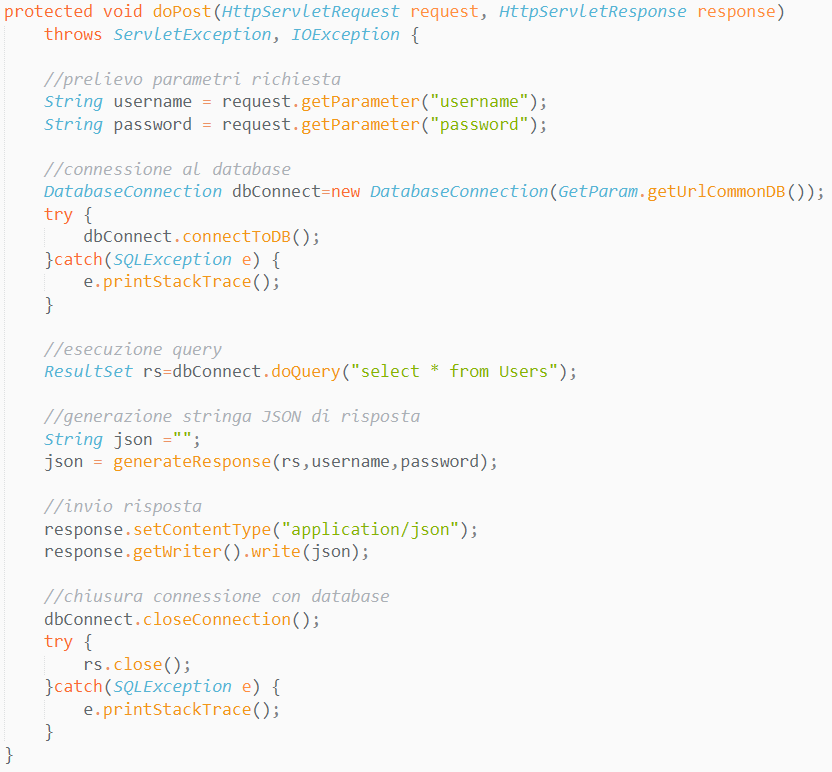
\includegraphics[height=11cm,width=\columnwidth]{codice/servlet} 
    \caption{Metodo \textit{doPost()} del \textit{servlet} che gestisce l'autenticazione}
\end{figure}

\subsubsection{Interrogazione del servizio \textit{web}}

Quando si implementa un \textit{servlet} concreto, \textit{eclipse} gli associa un \glossaryItem{end-point} in automatico. Tramite questo è possibile inviare richieste \textit{HTTP} ad uno specifico \textit{servlet} sul \textit{server}. L'\textit{end-point} assegnato da \textit{eclipse} è nella forma \textit{/NomeClasseServlet} e può essere cambiato dalle impostazioni dell'\textit{IDE}. Per rendere il servizio \textit{web} operativo, è necessario che ne venga effettuato il \textit{deploy} su \textit{Apache Tomcat} e che quest'ultimo venga  eseguito sul \textit{server Azure}. Una volta che il servizio \textit{web} diventa raggiungibile tramite la rete, è possibile iniziare ad effettuare richieste \textit{HTTP}. In \textit{moviORDER}, la struttura dell'\textit{URL} di una richiesta \textit{HTTP} è la seguente: \textit{http://indirizzo:porta/moviORDER/NomeServlet}, dove:
\begin{itemize}
	\item \textit{indirizzo}: è l'indirizzo del \textit{server} dove il servizio \textit{web} viene fatto girare:
	\item \textit{porta}: è la porta del \textit{server} dove il servizio \textit{web} viene fatto girare;
	\item \textit{NomeServlet}: è l'\textit{end-point} (\textit{servlet}) a cui si vuole inviare la richiesta \textit{HTTP}.
\end{itemize}

\textit{MoviORDER} effettua richieste \textit{HTTP} tramite \textit{AJAX} (\textit{Asynchronous JavaScript And XML}), ossia una tecnica per accedere ad un \textit{server web} da una pagina \textit{web}. \textit{AJAX} permette di leggere dati da un \textit{server web} dopo che una pagina è stata caricata, aggiornare una pagina \textit{web} senza il bisogno di dover ricaricare la stessa, e inviare dati ad un \textit{server web} in maniera del tutto trasparente all'utente. 

Nel progetto, \textit{AJAX} è stato implementato mediante \textit{JavaScript} con l'utilizzo dell'oggetto \textit{XMLHttpRequest}, il quale è supportato da tutti i \textit{browser} moderni e può essere utilizzato per scambiare dati con un \textit{server web} in maniera trasparente, ovvero senza il bisogno di dover ricaricare la pagina per cambiarne lo stato. La sintassi per creare un oggetto \textit{XMLHttpRequest} è la seguente:
\textit{var xhttp = new XMLHttpRequest();}. 

I metodi \textit{open()} e \textit{send()} permettono di inviare richieste \textit{HTTP} al servizio \textit{web}. In particolare, il metodo \textit{open()} permette di specificare la tipologia di richiesta da inviare tramite il passaggio di tre parametri:
	\begin{itemize}
		\item \textbf{metodo}: specifica il metodo utilizzato per inviare la richiesta \textit{HTTP}: \textit{GET} o \textit{POST};
		\item \textbf{url}: specifica l'indirizzo del \textit{server} a cui inviare la richiesta \textit{HTTP}. Nel caso del progetto, l'indirizzo comprende l'\textit{end-point} presso il quale la richiesta deve essere gestita;
		\item \textbf{asincrona/sincrona}: specifica se la richiesta è asincrona (\textit{true}) oppure sincrona (\textit{false}).
	\end{itemize}
Il metodo \textit{send(string)} permette invece l'invio di una richiesta \textit{HTTP} al servizio \textit{web}. Esso richiede il passaggio di una stringa contenente i parametri da inviare al \textit{server}. Poiché alcuni parametri potevano contenere caratteri accentati, è stato necessario utilizzare il metodo \textit{setRequestHeader()} per specificare la codifica dei caratteri. In questo modo si sono evitati errori di lettura/scrittura sul \textit{database} di \textit{moviORDER}. 

È importante far notare che tutte le richieste \textit{HTTP} inviate da \textit{moviORDER} al servizio \textit{web} sono asincrone, questo perché:
\begin{itemize}
	\item il codice sincrono non è raccomandato poiché \textit{JavaScript} ne stoppa l'esecuzione fino all'arrivo di una risposta da parte del \textit{server}. Inoltre, se quest'ultimo è occupato o lento, l'applicazione potrebbe attendere per un tempo prolungato;
	\item nei prossimi anni le richieste \textit{AJAX} sincrone saranno rimosse dallo standard \textit{web}. Scegliendo di utilizzare solamente richieste asincrone, si permetterà a \textit{moviORDER} di essere \glossaryItem{robusta} a questo cambiamento futuro.
\end{itemize} 

Per la gestione della risposta ricevuta dal \textit{server}, si sono utilizzate le seguenti proprietà dell'oggetto \textit{XMLHttpRequest}:
\begin{itemize}
	\item \textit{readyState}: contiene lo stato dell'oggetto. In particolare, per lo scopo del progetto, è interessante sapere che il valore 4 corrisponde ad una richiesta la cui risposta è pronta;
	\item  \textit{status}: contiene un messaggio sullo stato della richiesta. In particolare, per lo scopo del progetto, è interessante sapere che il valore 200 corrisponde al messaggio \textit{OK}, che nello standard \textit{web} rappresenta una richiesta \textit{HTTP} andata a buon fine;
	\item \textit{onreadystatechange}: definisce una funzione che deve essere eseguita quando la proprietà \textit{readyState} cambia valore;
	\item \textit{responseText}: incapsula la stringa di risposta ricevuta dal servizio \textit{web}. 
\end{itemize} 
Poiché la risposta del servizio \textit{web} è una stringa in formato \textit{JSON}, per effettuarne il \glossaryItem{parsing} si è dovuto convertirla in un oggetto \textit{JavaScript}, tramite l'utilizzo del metodo \textit{JSON.parse()}.

Viene di seguito fornito, a titolo d'esempio, il codice \textit{JavaScript} della logica applicativa che effettua una chiamata \textit{HTTP} all'\textit{end-point} che gestisce l'autenticazione. La funzione \textit{tryLogin()} viene eseguita nel momento in cui l'utente preme sul pulsante di \textit{login} presente nella schermata di autenticazione dell'applicazione.

\newpage

\begin{figure}[!h] 
    \centering 
    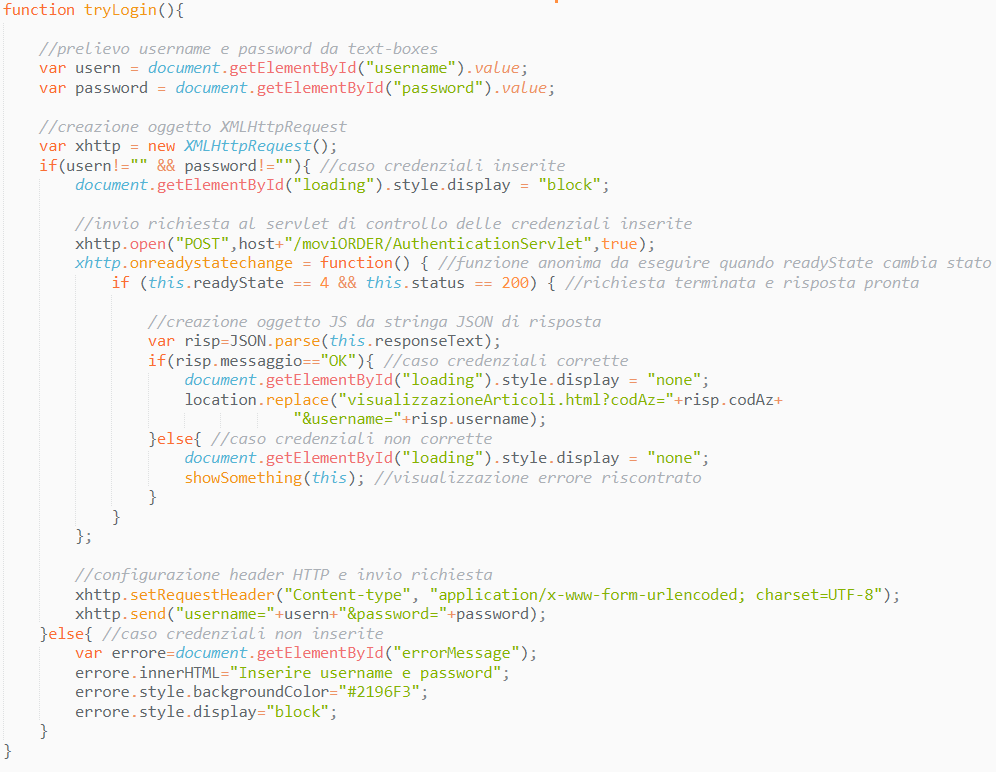
\includegraphics[width=\columnwidth]{codice/ajax} 
    \caption{Esempio di invio di una richiesta \textit{HTTP} tramite \textit{AJAX}}
\end{figure}

\subsubsection{\textit{API} del servizio \textit{web}} \label{api}

In questa sezione viene presentata l'\textit{API} del servizio \textit{web}. In particolare, per ogni \textit{end-point} vengono specificati:
\begin{itemize}
	\item \textbf{indirizzo}: indirizzo tramite il quale è possibile raggiungere l'\textit{end-point};
	\item \textbf{input}: costituito dai parametri che vengono inviati al servizio \textit{web} tramite una richiesta \textit{HTTP};
	\item \textbf{output}: costituito da una stringa in formato \textit{JSON} che presenta struttura diversa a seconda dell'\textit{end-point} che gestisce la richiesta;
	\item \textbf{descrizione}: breve descrizione del funzionamento dell'\textit{end-point}.
\end{itemize}

\myparagraph{Servizio di autenticazione}

\begin{itemize}
	\item \textbf{Indirizzo}: /AuthenticationServlet;
	\item \textbf{Input}: il \textit{servlet} richiede i seguenti parametri:
		\begin{itemize}
			\item \textit{username}: è la \textit{username} inserita dall'utente in fase di login;
			\item \textit{password}: è la \textit{password} inserita dall'utente in fase di login.
		\end{itemize}
	\item \textbf{Output}: le possibili risposte del \textit{servlet} sono le seguenti:
		\begin{itemize}
			\item codice azienda e \textit{username} dell'utente se \textit{username} e \textit{password} passati come parametro corrispondono ad un utente presente in \textit{database};
			\item un messaggio d'errore se le credenziali sono scorrette o l'utente è stato bloccato. 
		\end{itemize}
		\item \textbf{Descrizione}: questo \textit{servlet} rappresenta il servizio di autenticazione. Ricevuti i parametri, effettua la ricerca della \textit{username} nel \textit{database} e, nel caso in cui questa fosse presente, procede nel cercare la \textit{password} corrispondente.
\end{itemize}
% arrivato qui = sostituire tutti i "nel caso" in "se" e mettere tutto al presente
\myparagraph{Servizio di verifica di connessione con il \textit{database}}

\begin{itemize}
	\item \textbf{Indirizzo}: /CheckConnectionURL;
	\item \textbf{Input}: il \textit{servlet} richiede i seguenti parametri:
		\begin{itemize}
			\item \textit{codice azienda}: è il codice dell'azienda di cui si vuole verificare la presenza del \textit{database}.
		\end{itemize}
	\item \textbf{Output}: le possibili risposte del \textit{servlet} sono le seguenti:
		\begin{itemize}
			\item un messaggio positivo se il \textit{database} dell'azienda corrispondente al codice passato come parametro è raggiungibile;
			\item un messaggio negativo se il \textit{database} dell'azienda corrispondente al codice passato come parametro non è raggiungibile.
		\end{itemize}
	\item \textbf{Descrizione}: questo \textit{servlet} si occupa di controllare se un \textit{database} aziendale è raggiungibile effettuando una \textit{query} su di esso.
\end{itemize}

\myparagraph{Servizio di rimozione articoli in carrello}

\begin{itemize}
	\item \textbf{Indirizzo}: /DeleteSelectedItems;
	\item \textbf{Input}: il \textit{servlet} richiede i seguenti parametri:
		\begin{itemize}
			\item \textit{lista di codici articolo}: è la lista dei codici degli articoli che devono essere eliminati;
			\item \textit{username}: è la \textit{username} dell'utente che ha richiesto l'eliminazione degli articoli;
			\item \textit{path}: è la stringa di connessione al \textit{database} aziendale dell'utente autenticato.
		\end{itemize}
	\item \textbf{Output}: le possibili risposte del \textit{servlet} sono le seguenti:
		\begin{itemize}
			\item un messaggio positivo se la cancellazione è andata a buon fine;
			\item un messaggio negativo se la cancellazione non è andata a buon fine.
		\end{itemize}
	\item \textbf{Descrizione}: questo \textit{servlet} si occupa di eliminare dal \textit{database} aziendale dell'utente autenticato gli articoli che quest'ultimo ha richiesto di rimuovere dal carrello.
\end{itemize}

\myparagraph{Servizio di ricerca di un codice a barre}

\begin{itemize}
	\item \textbf{Indirizzo}: /FindArticleBarCode;
	\item \textbf{Input}: il \textit{servlet} richiede i seguenti parametri:
		\begin{itemize}
			\item \textit{codice a barre}: è il \textit{barcode} di un articolo del quale si vuole conoscere il codice;
			\item \textit{path}: è la stringa di connessione al \textit{database} aziendale dell'utente autenticato.
		\end{itemize}
	\item \textbf{Output}: le possibili risposte del \textit{servlet} sono le seguenti:
		\begin{itemize}
			\item codice articolo corrispondente al \textit{barcode} passato come parametro nel caso in cui il codice a barre corrisponde a quello di un articolo venduto dall'azienda;
			\item un messaggio negativo nel caso in cui il \textit{barcode} passato come parametro non corrisponde ad un articolo venduto dall'azienda.
		\end{itemize}
	\item \textbf{Descrizione}: questo \textit{servlet} si occupa di fornire il codice dell'articolo corrispondente al \textit{barcode} passato come parametro, effettuando la ricerca del codice a barre all'interno del \textit{database}.
\end{itemize}

\myparagraph{Servizio di ricerca di un codice articolo}

\begin{itemize}
	\item \textbf{Indirizzo}: /FindArticleCode;
	\item \textbf{Input}: il \textit{servlet} richiede i seguenti parametri:
		\begin{itemize}
			\item \textit{codice articolo}: è il codice o il \textit{barcode} di un articolo del quale si vuole verificare la presenza in \textit{database};
		\end{itemize}
	\item \textbf{Output}: le possibili risposte del \textit{servlet} sono le seguenti:
		\begin{itemize}
			\item codice dell'articolo nel caso in cui l'articolo è presente in \textit{database};
			\item un messaggio negativo nel caso in cui l'articolo non è presente in \textit{database}.
		\end{itemize}
	\item \textbf{Descrizione}: questo \textit{servlet} si occupa di fornire il codice dell'articolo corrispondente al codice o al \textit{barcode} ricevuto come parametro, effettuando la ricerca del codice articolo o del \textit{barcode} all'interno del \textit{database}.
\end{itemize}

\myparagraph{Servizio di prelievo delle informazioni di un articolo}

\begin{itemize}
	\item \textbf{Indirizzo}: /GetArticleDescNote;
	\item \textbf{Input}: il \textit{servlet} richiede i seguenti parametri:
		\begin{itemize}
			\item \textit{codice azienda}: è il codice dell'azienda di cui l'utente autenticato è cliente;
			\item \textit{codice articolo}: è il codice dell'articolo di cui si vogliono ottenere informazioni.
		\end{itemize}
	\item \textbf{Output}: questo \textit{servlet} può produrre un solo \textit{output}:
		\begin{itemize}
			\item descrizione, note, quantità minima ordinabile e \textit{step} di incremento quantità per l'articolo corrispondente al codice passato come parametro.
		\end{itemize}
	\item \textbf{Descrizione}: questo \textit{servlet} si occupa di fornire informazioni sull'articolo corrispondente al codice passato come parametro. 
\end{itemize}

\myparagraph{Servizio di prelievo degli articoli in carrello}

\begin{itemize}
	\item \textbf{Indirizzo}: /GetArticlesByUsername;
	\item \textbf{Input}: il \textit{servlet} richiede i seguenti parametri:
		\begin{itemize}
			\item \textit{codice azienda}: è il codice dell'azienda di cui l'utente autenticato è cliente;
			\item \textit{username}: è il nome utente dell'utente autenticato.
		\end{itemize}
	\item \textbf{Output}: le possibili risposte del \textit{servlet} sono le seguenti:
		\begin{itemize}
			\item lista degli articoli nel carrello dell'utente autenticato, dove per ogni articolo vengono restituiti la quantità ordinata, il codice e la descrizione;
			\item lista vuota nel caso in cui l'utente autenticato non presenta articoli in carrello.
		\end{itemize}
	\item \textbf{Descrizione}: questo \textit{servlet} si occupa di fornire la lista degli articoli in carrello delll'utente la quale \textit{username} è stata passata come parametro.
\end{itemize}

\myparagraph{Servizio di prelievo delle informazioni di un utente}

\begin{itemize}
	\item \textbf{Indirizzo}: /GetNameByUsername;
	\item \textbf{Input}: il \textit{servlet} richiede i seguenti parametri:
		\begin{itemize}
			\item \textit{path}: è la stringa di connessione al \textit{database} aziendale dell'utente autenticato;
			\item \textit{username}: è il nome utente dell'utente autenticato.
		\end{itemize}
	\item \textbf{Output}: questo \textit{servlet} può produrre un solo \textit{output}:
		\begin{itemize}
			\item nome e ragione sociale dell'utente autenticato e codice e descrizione del documento da generare se l'utente invia un ordine.
		\end{itemize}
	\item \textbf{Descrizione}: questo \textit{servlet} si occupa di fornire informazioni sull'utente la cui \textit{username} è stata passata come parametro.
\end{itemize}

\myparagraph{Servizio di prelievo delle informazioni di un articolo in carrello}

\begin{itemize}
	\item \textbf{Indirizzo}: /GetTmpArticleData;
	\item \textbf{Input}: il \textit{servlet} richiede i seguenti parametri:
		\begin{itemize}
			\item \textit{path}: è la stringa di connessione al \textit{database} aziendale dell'utente autenticato;
			\item \textit{codice articolo}: è il codice dell'articolo di cui si vogliono ottenere informazioni;
			\item \textit{username}: è il nome utente dell'utente autenticato.
		\end{itemize}
	\item \textbf{Output}: questo \textit{servlet} può produrre un solo \textit{output}:
		\begin{itemize}
			\item quantità e note dell'articolo in carrello corrispondente al codice articolo e all'utente passati come parametri.
		\end{itemize}
	\item \textbf{Descrizione}: questo \textit{servlet} si occupa di fornire informazioni riguardati uno specifico articolo nel carrello dell'utente la quale \textit{username} è stata passata come parametro.
\end{itemize}

\myparagraph{Servizio di inserimento/modifica articolo}

\begin{itemize}
	\item \textbf{Indirizzo}: /InsertUpdateArticle;
	\item \textbf{Input}: il \textit{servlet} richiede i seguenti parametri:
		\begin{itemize}
			\item \textit{path}: è la stringa di connessione al \textit{database} aziendale dell'utente autenticato;
			\item \textit{query}: è una stringa contenente la \textit{query} di inserimento/modifica di un articolo.
		\end{itemize}
	\item \textbf{Output}: le possibili risposte del \textit{servlet} sono le seguenti:
		\begin{itemize}
			\item un messaggio positivo se la \textit{query} va a buon fine;
			\item un messaggio negativo se la \textit{query} non va a buon fine.
		\end{itemize}
	\item \textbf{Descrizione}: questo \textit{servlet} si occupa di inserire o modificare un articolo nel carrello dell'utente autenticato. L'inserimento e la modifica avvengono mediante l'utilizzo dello stesso \textit{servlet} poiché la \textit{query} da eseguire sul \textit{database}, che può essere di tipo \textit{INSERT} o \textit{UPDATE}, viene passata come parametro.
\end{itemize}

\myparagraph{Servizio di invio di un ordine}

\begin{itemize}
	\item \textbf{Indirizzo}: /SendOrder;
	\item \textbf{Input}: il \textit{servlet} richiede i seguenti parametri:
		\begin{itemize}
			\item \textit{path}: è la stringa di connessione al \textit{database} aziendale dell'utente autenticato;
			\item \textit{codici articolo}: è la lista dei codici degli articoli che l'utente autenticato ha ordinato;
			\item \textit{username}: è il nome utente dell'utente autenticato;
			\item \textit{ragione sociale}: è la ragione sociale dell'utente autenticato;
			\item \textit{nome}: è il nome dell'utente autenticato;
			\item \textit{codice documento}: è il codice del documento che deve essere generato con l'ordine;
			\item \textit{data}: è la data d'invio dell'ordine;
			\item \textit{note}: sono le note inserite dall'utente in fase di invio ordine;
			\item \textit{codice azienda}: è il codice dell'azienda di cui l'utente autenticato è cliente.
		\end{itemize}
	\item \textbf{Output}: le possibili risposte del \textit{servlet} sono le seguenti:
		\begin{itemize}
			\item un messaggio positivo se l'ordine è stato inviato con successo;
			\item un messaggio negativo se l'ordine non è stato inviato con successo.
		\end{itemize}
	\item \textbf{Descrizione}: questo \textit{servlet} si occupa di registrare sul \textit{database} un ordine contenente gli articoli passati come parametro. Il resto dei parametri viene utilizzato per inviare una \textit{mail} di conferma all'utente autenticato e all'azienda presso cui l'utente ha ordinato.
\end{itemize}
\newpage
\subsection{\textit{JDBC}}

In questa sezione viene presentato l'utilizzo della \textit{Java Database Connectivity API} nella realizzazione del servizio \textit{web}.

\subsubsection{\textit{Driver JDBC}}

Un \textit{driver} \textit{JDBC} è una componente \textit{software} che permette ad un'applicazione \textit{Java} di interagire con un \textit{database}. Per supportare la connessione a singoli \textit{database}, \textit{JDBC} richiede i \textit{driver} per ogni \textit{database}. Il \textit{driver} permette la connessione con il \textit{database} e implementa il protocollo di trasferimento di \textit{query} e risultati tra \textit{client} e \textit{database}. Poiché nel progetto si è utilizzato \textit{SQL Server}, si sono dovuti utilizzare i \textit{driver} \textit{JDBC} per tale \textit{database}.

\subsubsection{Classe \textit{DatabaseConnection}} \label{dbconnect}

Per lo sviluppo del servizio \textit{web} è stata realizzata la classe \textit{DatabaseConnection}, appartenente al \textit{package} \textit{dbConnection}. Questa fornisce un'interfaccia utilizzabile per gestire l'interazione con un \textit{database} di tipo \textit{SQL Server}. In questa sezione vengono presentati i metodi di \textit{DatabaseConnection}.

\myparagraph{Costruttori}

La classe presenta i seguenti metodi costruttori:
\begin{itemize}
	\item \textit{public DatabaseConnection(String u, String user, String psw, String db)}: costruisce un oggetto \textit{DatabaseConnection} a partire dall'\textit{URL} del \textit{server} in cui è presente il \textit{database}, la \textit{username} e la \textit{password} di accesso, e il nome del \textit{database} al quale ci si desidera connettere;
	\item \textit{public DatabaseConnection(String dbConnectionString)}: costruisce un oggetto \textit{DatabaseConnection} a partire dalla stringa di connessione al \textit{database}.
\end{itemize}
Il formato di una stringa di connessione ad un \textit{database} è il seguente: \textit{indirizzoServer;databaseName=nomeDb;user=u;password=psw}, dove:
\begin{itemize}
	\item \textit{indirizzoServer}: è l'indirizzo pubblico del \textit{server} contenente il \textit{database} al quale ci si desidera connettere;
	\item \textit{nomeDb}: è il nome del \textit{database} al quale ci si desidera connettere;
	\item \textit{u}: è il nome utente per l'accesso al \textit{database};
	\item \textit{psw}: è la \textit{password} per l'accesso al \textit{database}.
\end{itemize}
Viene di seguito presentato, a titolo d'esempio, il codice \textit{Java} che implementa il metodo \textit{public DatabaseConnection(String dbConnectionString)}. Esso si occupa di \textit{splittare} la stringa di connessione passata come parametro per ottenere i dati utili alla costruzione dell'oggetto \textit{DatabaseConnection}.
\newpage
\begin{figure}[!h] 
    \centering 
    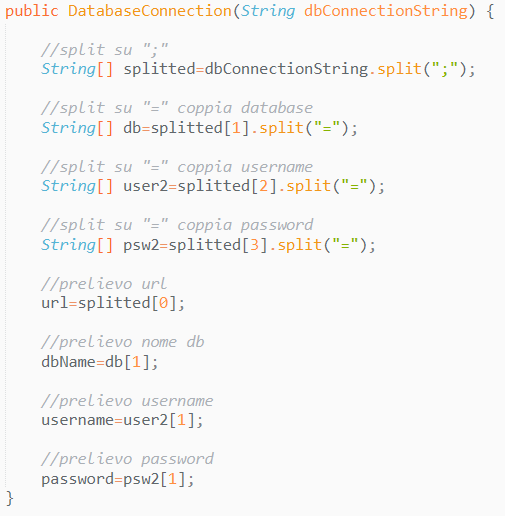
\includegraphics[height=9cm,width=0.8\columnwidth]{codice/databaseCostruttore} 
    \caption{Metodo costruttore della classe \textit{DatabaseConnection}}
\end{figure}

\myparagraph{Metodo \textit{connectToDb()}}

Tale metodo si occupa di instaurare la connessione con il \textit{database} desiderato. Per far questo, configura i \textit{driver} \textit{JDBC} e costruisce l'\textit{URL} di connessione al \textit{database}. Il metodo solleva un'eccezione di tipo \textit{ClassNotFoundException} se classe utilizzata per i \textit{driver} \textit{JDBC} è inesistente o non è stata importata all'interno del progetto. Viene di seguito fornito, a titolo d'esempio, il codice del metodo \textit{connectToDb()}.

\begin{figure}[!h] 
    \centering 
    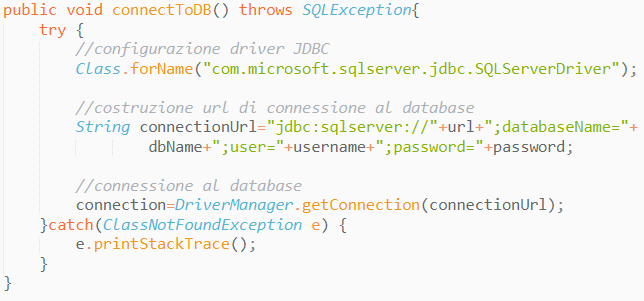
\includegraphics[width=\columnwidth]{codice/connessionedb} 
    \caption{Metodo \textit{connectToDb()} della classe \textit{DatabaseConnection}}
\end{figure}
\newpage
\myparagraph{Altri metodi}

La classe \textit{DatabaseConnection} presenta altri metodi di complessità inferiore, per i quali viene presentata solamente una breve descrizione:
\begin{itemize}
	\item \textit{doQuery(query)}: permette di eseguire una \textit{query} di tipo \textit{SELECT} sul \textit{database}. Restituisce un \textit{ResultSet} contenente il risultato della \textit{query};
	\item \textit{doUpdateQuery(query)}: permette di eseguire una \textit{query} di tipo \textit{INSERT}, \textit{UPDATE} o \textit{DELETE} sul \textit{database}. Restituisce il numero di righe inserite, modificate o cancellate;
	\item \textit{closeConnection()}: permette di eseguire il processo di disconnessione dal \textit{database}.
\end{itemize}

\subsection{Classi utilità}

Per lo sviluppo del servizio \textit{web} è stato necessario scrivere due classi utilità, che appartengono al \textit{package} \textit{utility}. Viene di seguito fornita una breve descrizione della loro implementazione.

\subsubsection{Classe \textit{GetParam}}

La classe \textit{GetParam} si occupa di restituire un campo statico contenente la stringa di connessione al \textit{database} \textit{CommonDb}. Questa viene frequentemente utilizzata all'interno del servizio \textit{web}, quindi si è deciso di inserirla in un unico punto del codice, in modo da evitare la modifica di più \textit{file} nel caso in cui venga modificata.

\subsubsection{Classe \textit{MailUtility}}

La classe \textit{MailUtility} fornisce un'interfaccia per l'invio di \textit{e-mail}. È stata implementata per inviare una \textit{mail} di conferma all'utente autenticato e alla sua azienda quando un ordine viene registrato. La classe presenta un costruttore che richiede i parametri per la configurazione di un \glossaryItem{server SMTP}:
\begin{itemize}
	\item \textbf{host}: è l'indirizzo dell'\textit{host} su cui è installato il \textit{server SMTP};
	\item \textbf{post}: è la porta dell'\textit{host} su cui è installato il \textit{server SMTP};
	\item \textbf{\textit{username}}: è il nome utente di accesso al \textit{server SMTP};
	\item \textbf{\textit{password}}: è la \textit{password} di accesso al \textit{server SMTP}.
\end{itemize}
Il metodo \textit{sendMail()} si occupa di configurare e inviare una \textit{mail} all'utente che ha effettuato l'ordine e alla sua azienda. Per far questo, il metodo richiede:
\begin{itemize}
	\item indirizzo \textit{e-mail} dell'utente;
	\item indirizzo \textit{e-mail} dell'azienda;
	\item indirizzo \textit{e-mail} del mittente;
	\item oggetto dell'\textit{e-mail};
	\item testo dell'\textit{e-mail}: è una tabella scritta in codice \textit{HTML} contenente i dati degli articoli ordinati.
\end{itemize}
Viene di seguito fornito, a titolo d'esempio, il codice \textit{Java} che implementa il metodo \textit{sendMail()}.

\newpage

\begin{figure}[!h] 
    \centering 
    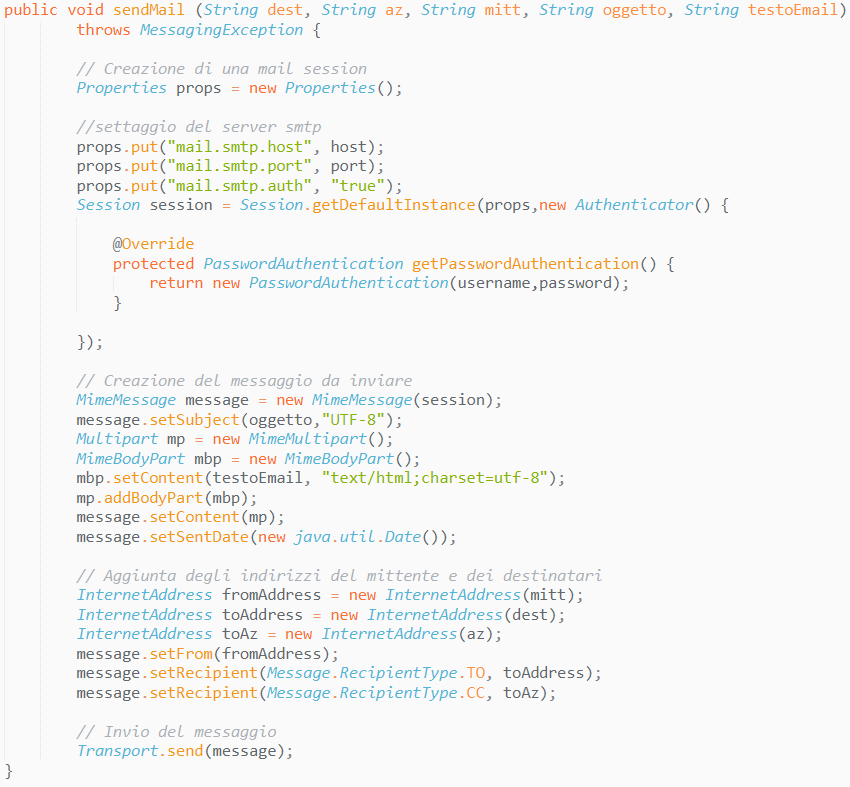
\includegraphics[width=\columnwidth]{codice/mail} 
    \caption{Metodo \textit{sendMail()} della classe \textit{MailUtility}}
\end{figure}
%qui
\section{Logica applicativa}

In questa sezione vengono presentati gli aspetti più interessanti riguardanti la codifica della logica applicativa di \textit{moviORDER}. La sezione si incentra sui meccanismi di integrazione dei \textit{plugin} \textit{PhoneGap} con il codice \textit{Javascript} della logica applicativa.

\subsection{\textit{Plugin} di \textit{PhoneGap}}

Un \textit{plugin} è un pacchetto di codice che permette al visualizzatore \textit{web} di \textit{Cordova}, il quale renderizza l'applicazione, di comunicare con la piattaforma nativa sulla quale viene eseguito. I \textit{plugin} forniscono accesso alle funzionalità del dispositivo che normalmente non sono disponibili per le applicazioni \textit{web-based}. Tutte le \textit{API} di \textit{Cordova} sono implementate tramite \textit{plugin}. Essi sono composti da un'unica interfaccia \textit{JavaScript} che astrae le differenti implementazioni in codice nativo delle funzionalità fornite dal \textit{plugin}. In fase di \textit{build} dell'applicazione, il codice \textit{JavaScript} dei \textit{plugin} viene convertito nel codice nativo della piattaforma sulla quale si sta distribuendo l'applicazione.

\subsection{Installazione dei \textit{plugin}}

Tramite \textit{PhoneGap CLI}, interfaccia a linea di comando precedentemente descritta, è possibile aggiungere \textit{plugin} alla configurazione del progetto \textit{PhoneGap}. È sufficiente lanciare la \textit{CLI} dalla cartella principale del progetto ed eseguire il comando \textit{phonegap plugin add nomePlugin}, dove \textit{nomePlugin} è il nome del \textit{plugin} che si desidera scaricare ed installare (es. \textit{cordova-plugin-whitelist}).

\subsection{Premesse all'utilizzo dei \textit{plugin}}

Per poter utilizzare efficacemente i \textit{plugin}, è necessario predisporre il codice \textit{JavaScript} al loro utilizzo. In particolare, sono necessari due accorgimenti che vengono di seguito presentati.

\subsubsection{Inclusione di \textit{cordova.js}}

Ogni \textit{file} della logica applicativa che utilizza dei \textit{plugin} deve includere il file \textit{cordova.js}. Questo \textit{file} \textit{JavaScript} permette il funzionamento dei \textit{plugin} utilizzati all'interno della logica. Se si utilizzasse un \textit{plugin} senza aver importato tale \textit{file}, la \textit{console} darebbe il seguente errore: ``\textit{Cordova in not available, Make sure to include cordova.js}''.

\subsubsection{Evento \textit{deviceready}}

L'evento \textit{deviceready} è essenziale in ogni applicazione \textit{PhoneGap}, poiché segnala il corretto caricamento delle \textit{API} di \textit{Cordova} sul dispositivo. Se l'evento non venisse atteso prima di utilizzare un \textit{plugin}, si rischierebbe che l'applicazione effettui chiamate a funzioni \textit{JavaScript} di \textit{Cordova} prima che il corrispondente codice nativo per il dispositivo diventi disponibile. L'evento \textit{deviceready} viene lanciato nel momento in cui \textit{Cordova} è stato completamente caricato. Quindi, dopo aver atteso l'evento, è possibile effettuare chiamate alle \textit{API} di \textit{Cordova} in completa sicurezza. Per attendere l'evento è sufficiente inserire un \textit{listener} nel codice \textit{JavaScript}. Viene di seguito fornito, a scopo illustrativo, un esempio di codice \textit{JavaScript} che implementa l'attesa di tale evento.

\begin{figure}[!h] 
    \centering 
    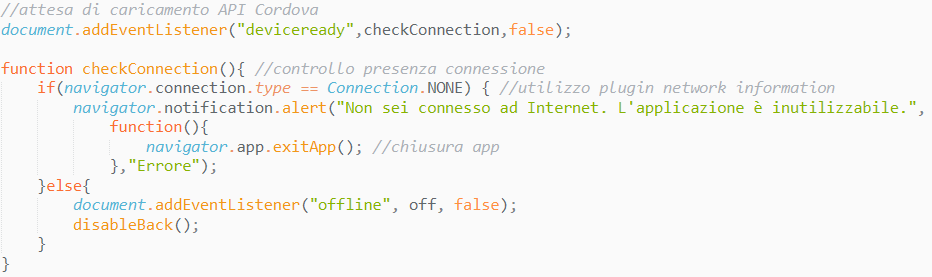
\includegraphics[width=\columnwidth]{codice/deviceready} 
    \caption{Esempio di codice \textit{JavaScript} che attende l'evento \textit{deviceready}}
\end{figure}

\subsection{Plugin utilizzati}

In questa sezione vengono presentati i \textit{plugin} \textit{PhoneGap} utilizzati nella realizzazione della logica applicativa di \textit{moviORDER}. Per ogni \textit{plugin} vengono messi in evidenzia vantaggi, svantaggi (se presenti) e un esempio di utilizzo.

\subsubsection{\textit{Dialogs plugin}}

Il \textit{plugin} \textit{dialogs} fornisce accesso all'interfaccia grafica nativa degli elementi \textit{dialog}, tramite l'utilizzo dell'oggetto \textit{navigator.notification}. Questo \textit{plugin} è stato utilizzato per convertire gli \textit{alert box} delle usuali pagine \textit{web} in \textit{dialog} nativi per l'ambiente \textit{mobile}. Si sono utilizzati i seguenti metodi:
\begin{itemize}
	\item \textit{alert()}: visualizza un \textit{dialog} con contente messaggio di allerta preimpostato. Il metodo richiede i seguenti parametri:
	\begin{itemize}
		\item \textit{message}: è il messaggio visualizzato nel \textit{dialog};
		\item \textit{callback}: è una \glossaryItem{funzione anonima} di \textit{callback} da eseguire quando viene premuto il pulsante nel \textit{dialog};
		\item \textit{title}: è il titolo del \textit{dialog};
		\item \textit{buttonName}: è l'etichetta del pulsante nel \textit{dialog}.
	\end{itemize}
	\item \textit{confirm()}: visualizza un \textit{dialog} per chiedere conferma di un'azione. Il metodo richiede i seguenti parametri:
	\begin{itemize}
		\item \textit{message}: è il messaggio visualizzato nel \textit{dialog} di conferma;
		\item \textit{callback}: è una funzione anonima di \textit{callback} da eseguire se il bottone di conferma viene premuto;
		\item \textit{title}: è il titolo del \textit{dialog} di conferma;
		\item \textit{buttonLabels}: sono le etichette dei vari bottoni presenti nel \textit{dialog} di conferma. Solitamente sono ``OK'' e ``Annulla''.
	\end{itemize}
\end{itemize}

Senza l'utilizzo di questo \textit{plugin} non si sarebbe potuto modificare il titolo e i bottoni del \textit{dialog}, poiché per motivi di sicurezza \textit{JavaScript} non permette tale modifica. Inoltre, la visualizzazione del \textit{dialog} non sarebbe stata quella desiderata, ovvero la visualizzazione nativa. 

Vengono di seguito forniti, a scopo illustrativo, un esempio di codice \textit{JavaScript} che non utilizza il \textit{plugin} e un esempio che lo utilizza. Per ognuno degli esempi viene mostrato uno \textit{screenshot} dell'\textit{output} risultante che, nel primo caso sarà un comune \textit{alert}, mentre nel secondo un \textit{dialog} nativo.

\begin{figure}[!h] 
    \centering 
    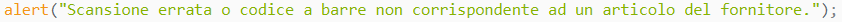
\includegraphics[width=\columnwidth]{codice/alert} 
    \caption{Esempio di codice \textit{JavaScript} che non utilizza il \textit{plugin} \textit{dialogs}}
\end{figure}

\newpage

\begin{figure}[!h] 
    \centering 
    \includegraphics[width=0.4\columnwidth]{codice/imgalert} 
    \caption{Esempio di visualizzazione scorretta (\textit{alert})}
\end{figure}

\begin{figure}[!h] 
    \centering 
    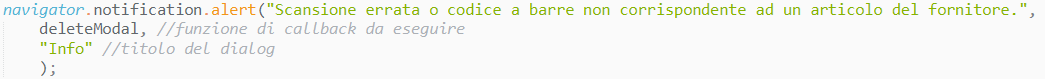
\includegraphics[width=\columnwidth]{codice/dialog} 
    \caption{Esempio di codice \textit{JavaScript} che utilizza il \textit{plugin} \textit{dialogs}}
\end{figure}

\begin{figure}[!h] 
    \centering 
    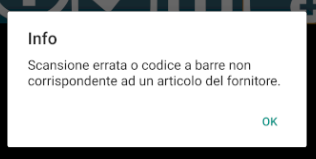
\includegraphics[width=0.4\columnwidth]{codice/imgDialog} 
    \caption{Esempio di visualizzazione corretta (\textit{dialog})}
\end{figure}

\subsubsection{\textit{Network information plugin}}

Il \textit{plugin} \textit{network information} fornisce un'implementazione moderna della \textit{Network Information API}, la quale consente di ottenere informazioni riguardanti la rete cellulare e il \textit{Wi-Fi} del dispositivo, e permette di capire se il \textit{device} presenta una connessione ad \textit{Internet}. Più precisamente, il \textit{plugin} fornisce un'interfaccia \textit{JavaScript} che astrae il codice nativo utilizzato per monitorare la rete del dispositivo. \textit{Navigator.connection} è l'oggetto che permette di acquisire le informazioni appena descritte. La proprietà \textit{type} è stata utilizzata per comprendere in modo veloce lo stato della connessione del dispositivo e la tipologia di connessione attiva. Essa può assumere i seguenti valori:
\begin{itemize}
	\item \textit{Connection.UNKNOWN}: tipologia di rete sconosciuta;
	\item \textit{Connection.ETHERNET}: dispositivo connesso alla rete via cavo \textit{ethernet};
	\item \textit{Connection.WIFI}: dispositivo connesso ad una rete \textit{Wi-Fi};
	\item \textit{Connection.CELL\_2G}: dispositivo connesso ad una rete cellulare di tipo \textit{2G};
	\item \textit{Connection.CELL\_3G}: dispositivo connesso ad una rete cellulare di tipo \textit{3G};
	\item \textit{Connection.CELL\_4G}: dispositivo connesso ad una rete cellulare di tipo \textit{4G};
	\item \textit{Connection.CELL}: dispositivo connesso ad una rete cellulare la cui tipologia non è identificabile;
	\item \textit{Connection.NONE}: dispositivo non connesso alla rete.
\end{itemize}
Un limite di questa proprietà è presente in ambiente \textit{iOS}, infatti non è possibile identificare nessun tipo di rete cellulare alla quale il dispositivo è connesso. Per questo, su \textit{iOS}, si è dovuta utilizzare la proprietà \textit{onLine} dell'oggetto \textit{navigator}.

All'oggetto \textit{navigator.connection} sono associate due tipologie di evento:
\begin{itemize}
	\item \textit{offline}: viene lanciato quando un dispositivo precedentemente collegato ad \textit{Internet} perde la connessione e quindi l'applicazione non è più in grado di accedere alla rete. In particolare, viene lanciato esattamente quando il valore della proprietà \textit{type} diventa \textit{Connection.NONE};
	\item \textit{online}: viene lanciato quando un dispositivo precedentemente scollegato dalla rete riceve la connessione permettendo all'applicazione di accedere ad \textit{Internet}. In particolare, viene lanciato esattamente quando il valore della proprietà \textit{type} cambia da \textit{NONE} ad un altro valore.
\end{itemize}
Il \textit{plugin} \textit{network information} è stato utilizzato per chiudere \textit{moviORDER} nel caso in cui venga aperta mentre il dispositivo è \textit{offline}. L'evento \textit{offline} ha permesso di visualizzare messaggi relativi allo stato della connessione. Più precisamente, se il dispositivo perde la connessione durante l'utilizzo dell'applicazione, viene visualizzato un messaggio che notifica l'inutilizzabilità della stessa.

Vengono di seguito forniti, a scopo illustrativo, degli esempi di codice \textit{JavaScript} che utilizzano la proprietà \textit{type} e l'evento \textit{offline} dell'oggetto \textit{network.connection}.

\begin{figure}[!h] 
    \centering 
    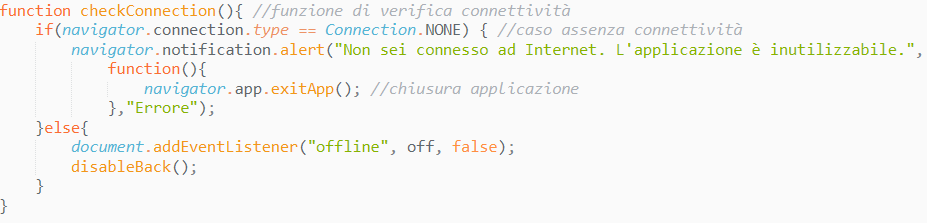
\includegraphics[width=\columnwidth]{codice/type} 
    \caption{Esempio di utilizzo della proprietà \textit{type}}
\end{figure}

\begin{figure}[!h] 
    \centering 
    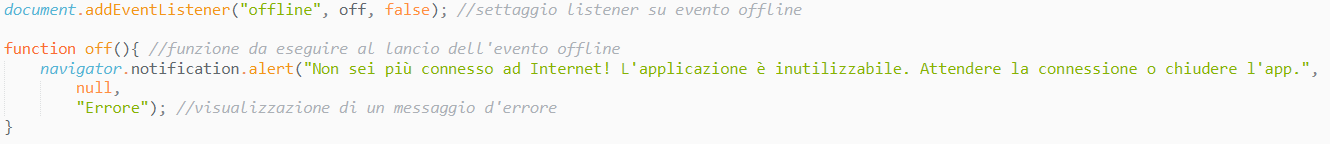
\includegraphics[width=\columnwidth]{codice/offline} 
    \caption{Esempio di utilizzo dell'evento \textit{offline}}
\end{figure}

\subsubsection{\textit{Barcode scanner plugin}}

Il \textit{plugin} \textit{barcode scanner} fornisce un'interfaccia \textit{JavaScript} per effettuare la scansione di un codice a barre da un qualsiasi dispositivo dotato di fotocamera. Per utilizzare il \textit{plugin} è sufficiente invocare il metodo \textit{scan(success, fail, settings)} sull'oggetto \textit{cordova.plugin.barcodeScanner}. \textit{Success} è una funzione di \textit{callback} che viene eseguita quando la scansione del \textit{barcode} va a buon fine, mentre \textit{Fail} viene eseguita quando la scansione fallisce. \textit{Settings} è una variabile contenente le seguenti impostazioni per l'utilizzo del \textit{plugin}:
\begin{itemize}
	\item \textit{preferFrontCamera}: permette di impostare la fotocamera frontale come predefinita per la scansione del codice a barre;
	\item \textit{showFlipCameraButton}: permette di visualizzare il bottone per cambiare fotocamera;
	\item \textit{showTorchButton}: permette di visualizzare il bottone per l'attivazione del \textit{flash};
	\item \textit{torchOn}: permette di attivare il \textit{flash} quando viene effettuata una scansione;
	\item \textit{saveHistory}: permette di salvare la cronologia dei codici scansionati;
	\item \textit{prompt}: permette di visualizzare un messaggio per aiutare l'utente ad eseguire la scansione;
	\item \textit{resultDisplayDuration}: permette di visualizzare il risultato della scansione per un certo periodo di tempo;
	\item \textit{formats}: permette di impostare la tipologia di codici a barre che devono essere captati;
	\item \textit{orientation}: permette di impostare l'orientamento del dispositivo (\textit{portrait} o \textit{landscape});
	\item \textit{disableAnimations}: permette di disabilitare le animazioni visualizzate durante la scansione del codice a barre;
	\item \textit{disableSuccessBeep}: permette di disabilitare il suono acustico emesso quando un codice viene captato.
\end{itemize}
Per poter utilizzare il \textit{plugin} in ambiente \textit{iOS} è necessario aggiungere una \textit{NSCameraUsageDescription} al \textit{file} \textit{Info.plist}, ossia una proprietà descrive la ragione per cui l'applicazione deve accedere alla fotocamera del dispositivo.

Il \textit{plugin} ha funzionato correttamente in ambiente \textit{Android}, ma ha presentato alcuni problemi su \textit{iOS}. Nei dispositivi dotati di fotocamera mediocre, le scansioni richiedevano più tempo del previsto (alcuni minuti). Per risolvere il problema si è dovuto modificare il codice nativo della versione \textit{iOS} dell'applicazione. Esso differenziava il processo di scansione a seconda della qualità rilevata per la fotocamera del dispositivo. Per cellulari dotati di fotocamera mediocre veniva fatta una valutazione troppo ottimistica, e per questo si è dovuto modificare il codice in modo da rendere il processo di scansione uguale per tutte le fotocamere. Dopo vari test si è potuto osservare che la soluzione migliore stava nell'utilizzo del processo di scansione per fotocamere di qualità media. Viene di seguito fornito, a scopo illustrativo, il codice \glossaryItem{Objective-C++} che si occupa di settare il processo di scansione.

\begin{figure}[!h] 
    \centering 
    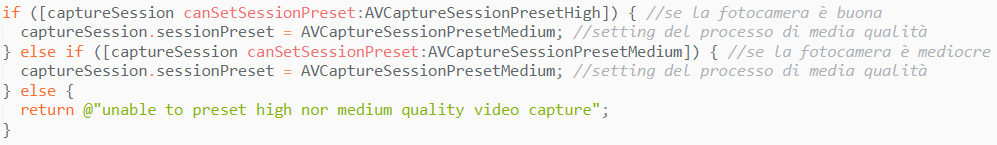
\includegraphics[width=\columnwidth]{codice/scan} 
    \caption{Codice \textit{Objective-C++} per il settaggio del processo di scansione}
\end{figure}

\newpage

Viene di seguito fornito, a scopo illustrativo, il codice \textit{JavaScript} della logica applicativa che utilizza il \textit{plugin} \textit{barcode scanner}.

\begin{figure}[!h] 
    \centering 
    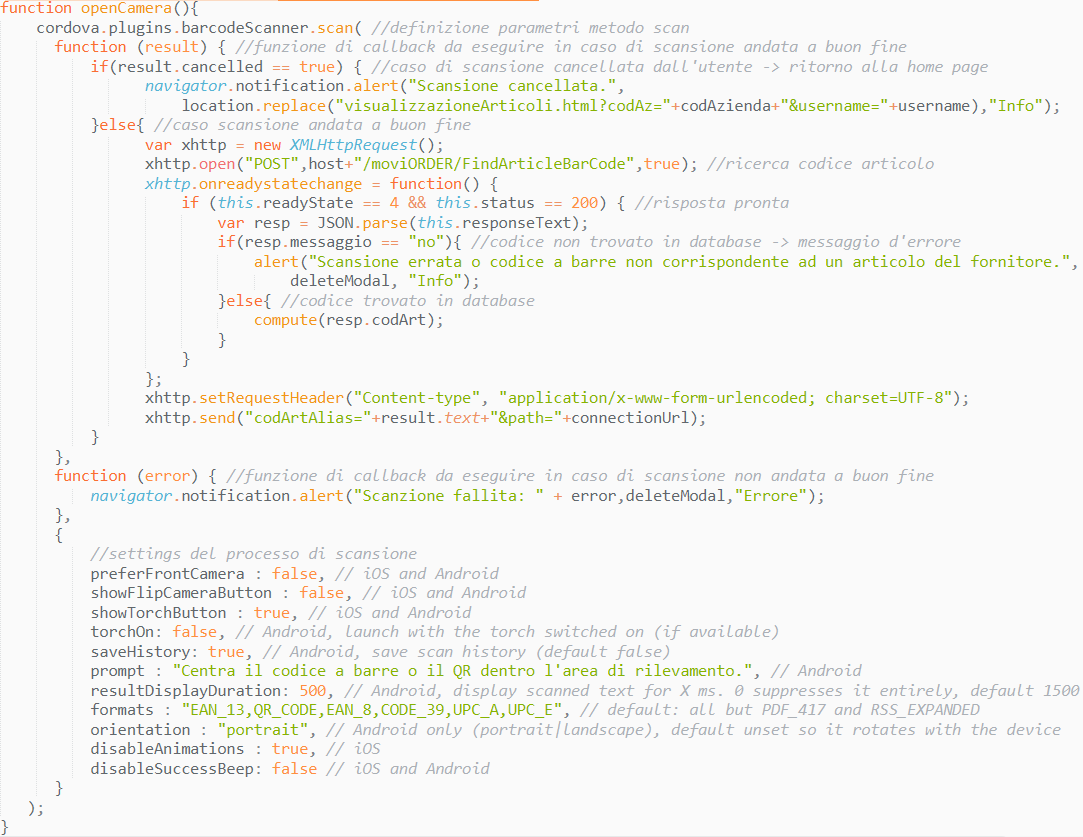
\includegraphics[width=\columnwidth]{codice/scan2} 
    \caption{Codice \textit{JavaScript} che utilizza il \textit{plugin} \textit{barcode scanner}}
\end{figure}

\newpage

\section{Interfaccia grafica}

In questa sezione vengono presentati gli aspetti più interessanti riguardanti la codifica dell'interfaccia grafica di \textit{moviORDER}. In particolare, vengono presentate le possibili interazioni dell'utente con le interfacce. Nell'ultima sezione vengono illustrate delle considerazioni sullo sviluppo dell'interfaccia.

\subsection{Schermata di \textit{login}}

\begin{figure}[!h] 
    \centering 
    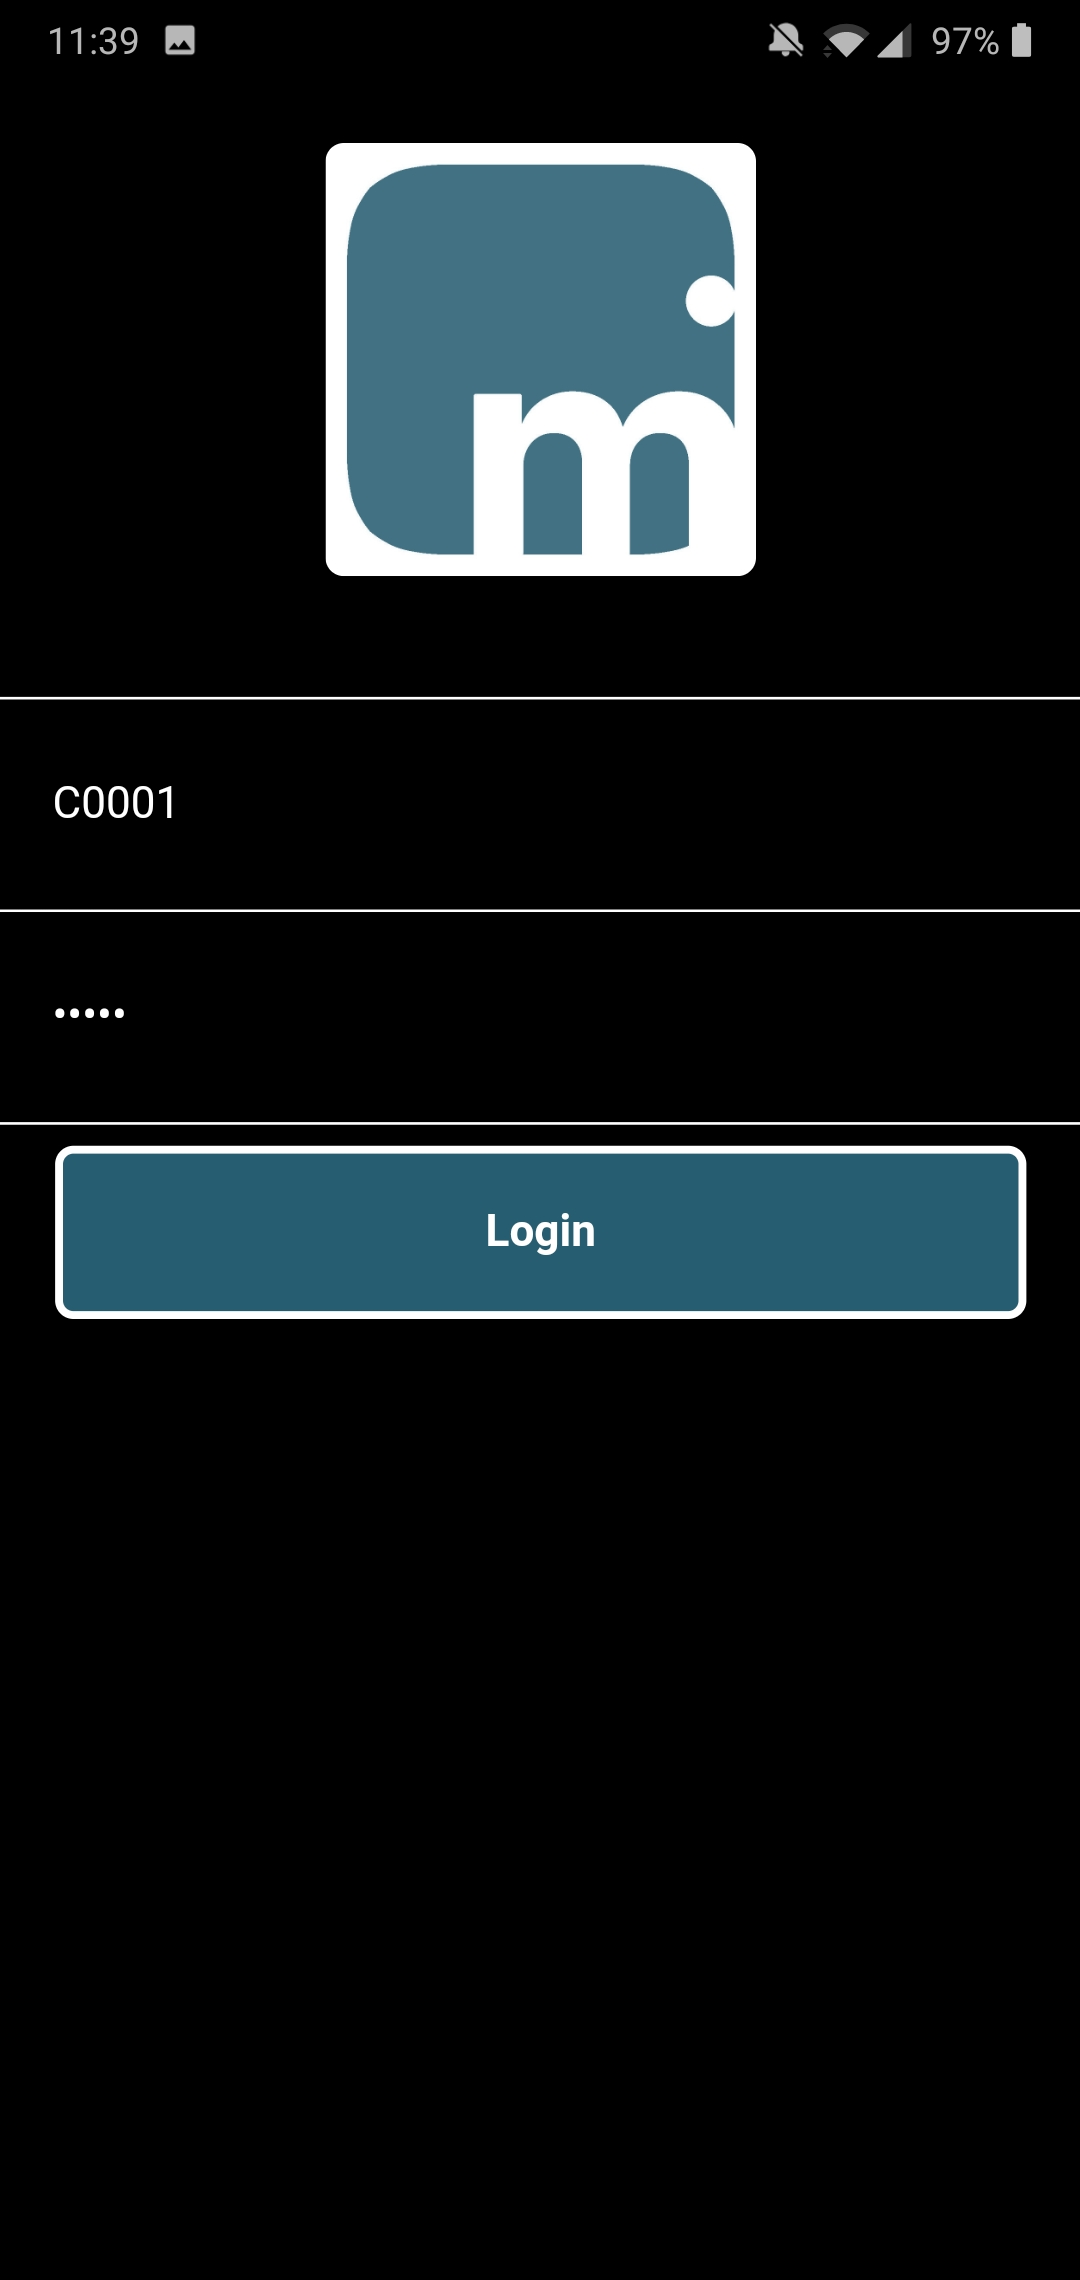
\includegraphics[width=0.4\columnwidth]{interfaccia/login} 
    \caption{Schermata di login}
\end{figure}

Tramite la schermata di \textit{login}, un qualsiasi utente in possesso di credenziali di accesso può accedere a \textit{moviORDER}. Per tentare l'accesso è necessario inserire \textit{username} e \textit{password} e, successivamente, premere sul pulsante di \textit{login}. Se l'utente inserisce credenziali corrette verrà aperta la \textit{home page} dell'applicazione, mentre se le credenziali non dovessero essere corrette verrà visualizzato un messaggio d'errore. Quest'ultimo è esplicativo dell'errore riscontrato, che può essere uno dei seguenti:
\begin{itemize}
	\item le credenziali non sono state inserite;
	\item la \textit{username} inserita è inesistente;
	\item la \textit{password} inserita non è corretta;
	\item le credenziali inserite sono corrette ma l'utente è stato bloccato dall'azienda.
\end{itemize}

\subsection{\textit{Home page}}

\begin{figure}[!h] 
    \centering 
    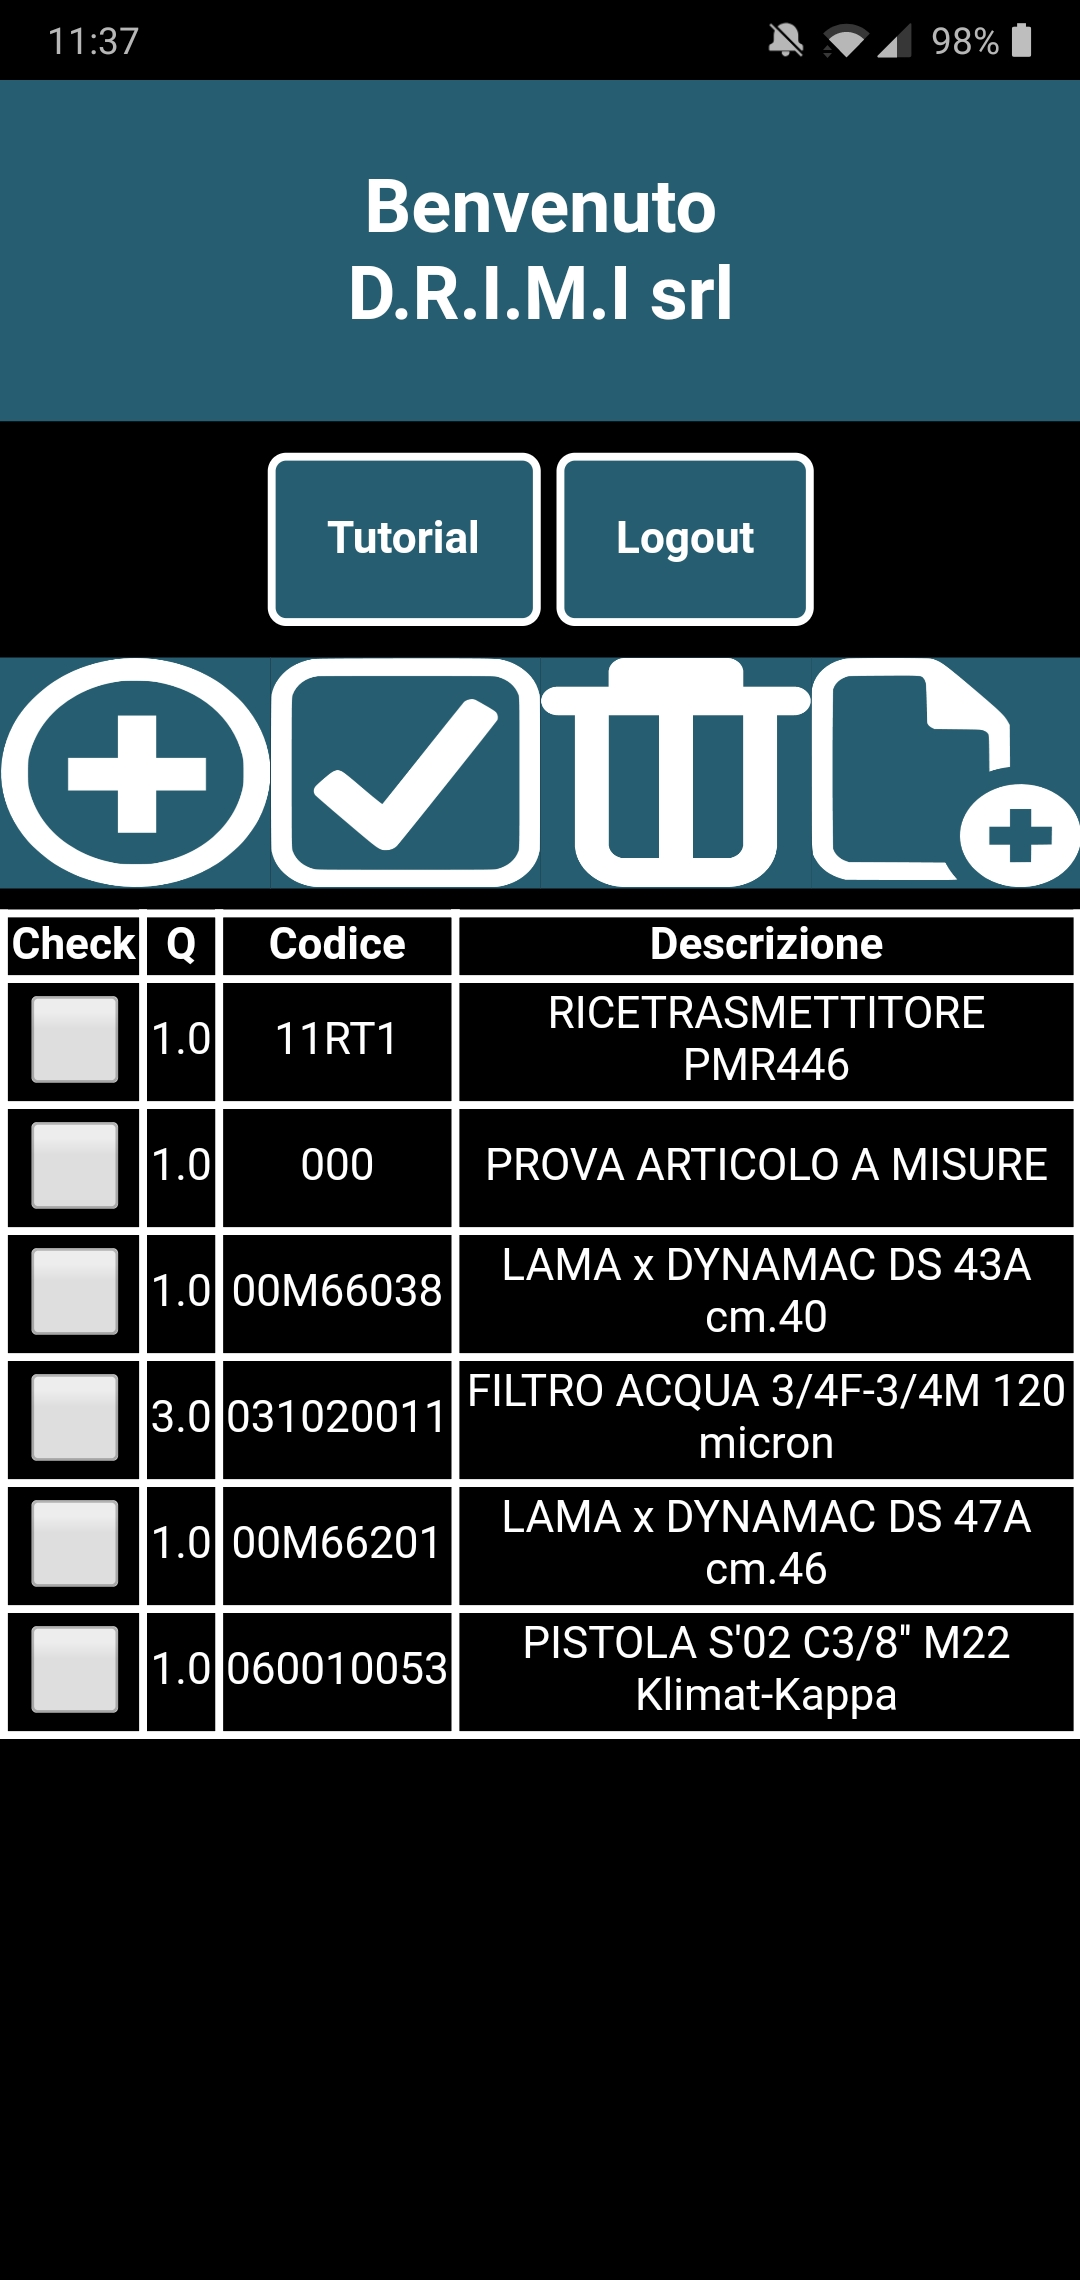
\includegraphics[width=0.4\columnwidth]{interfaccia/home} 
    \caption{\textit{Home page}}
\end{figure}

La \textit{home page} racchiude le funzionalità di \textit{moviORDER} dedicate all'utente autenticato. A partire dall'alto e proseguendo verso il basso, l'interfaccia presenta le seguenti parti:
\begin{itemize}
	\item \textbf{messaggio di benvenuto}: contiene la ragione sociale dell'utente;
	\item \textbf{pulsante \textit{tutorial}}: permette di visualizzare il \textit{tutorial} dell'applicazione;
	\item \textbf{pulsante \textit{logout}}: permette di effettuare il \textit{logout} dall'applicazione;
	\item \textbf{pulsante di aggiunta articolo}: permette di accedere al \textit{modal} per l'aggiunta di un articolo in carrello; 
	\item \textbf{pulsante di selezione/deselezione multipla di articoli}: permette di selezionare/deselezionare tutti gli articoli in carrello;
	\item \textbf{pulsante di eliminazione articoli}: permette di rimuovere dal carrello gli articoli selezionati;
	\item \textbf{pulsante di invio ordine}: permette di accedere al \textit{modal} per l'invio di un ordine;
	\item \textbf{carrello}: ogni articolo in carrello presenta:
	\begin{itemize}
		\item una \textit{checkbox} per selezionare/deselezionare l'articolo;
		\item un'indicazione sulla quantità di pezzi ordinati;
		\item il codice dell'articolo;
		\item una breve descrizione dell'articolo.
	\end{itemize}
\end{itemize}

\subsection{\textit{Modal} per l'aggiunta di un articolo}

\begin{figure}[!h] 
    \centering 
    	\subfloat{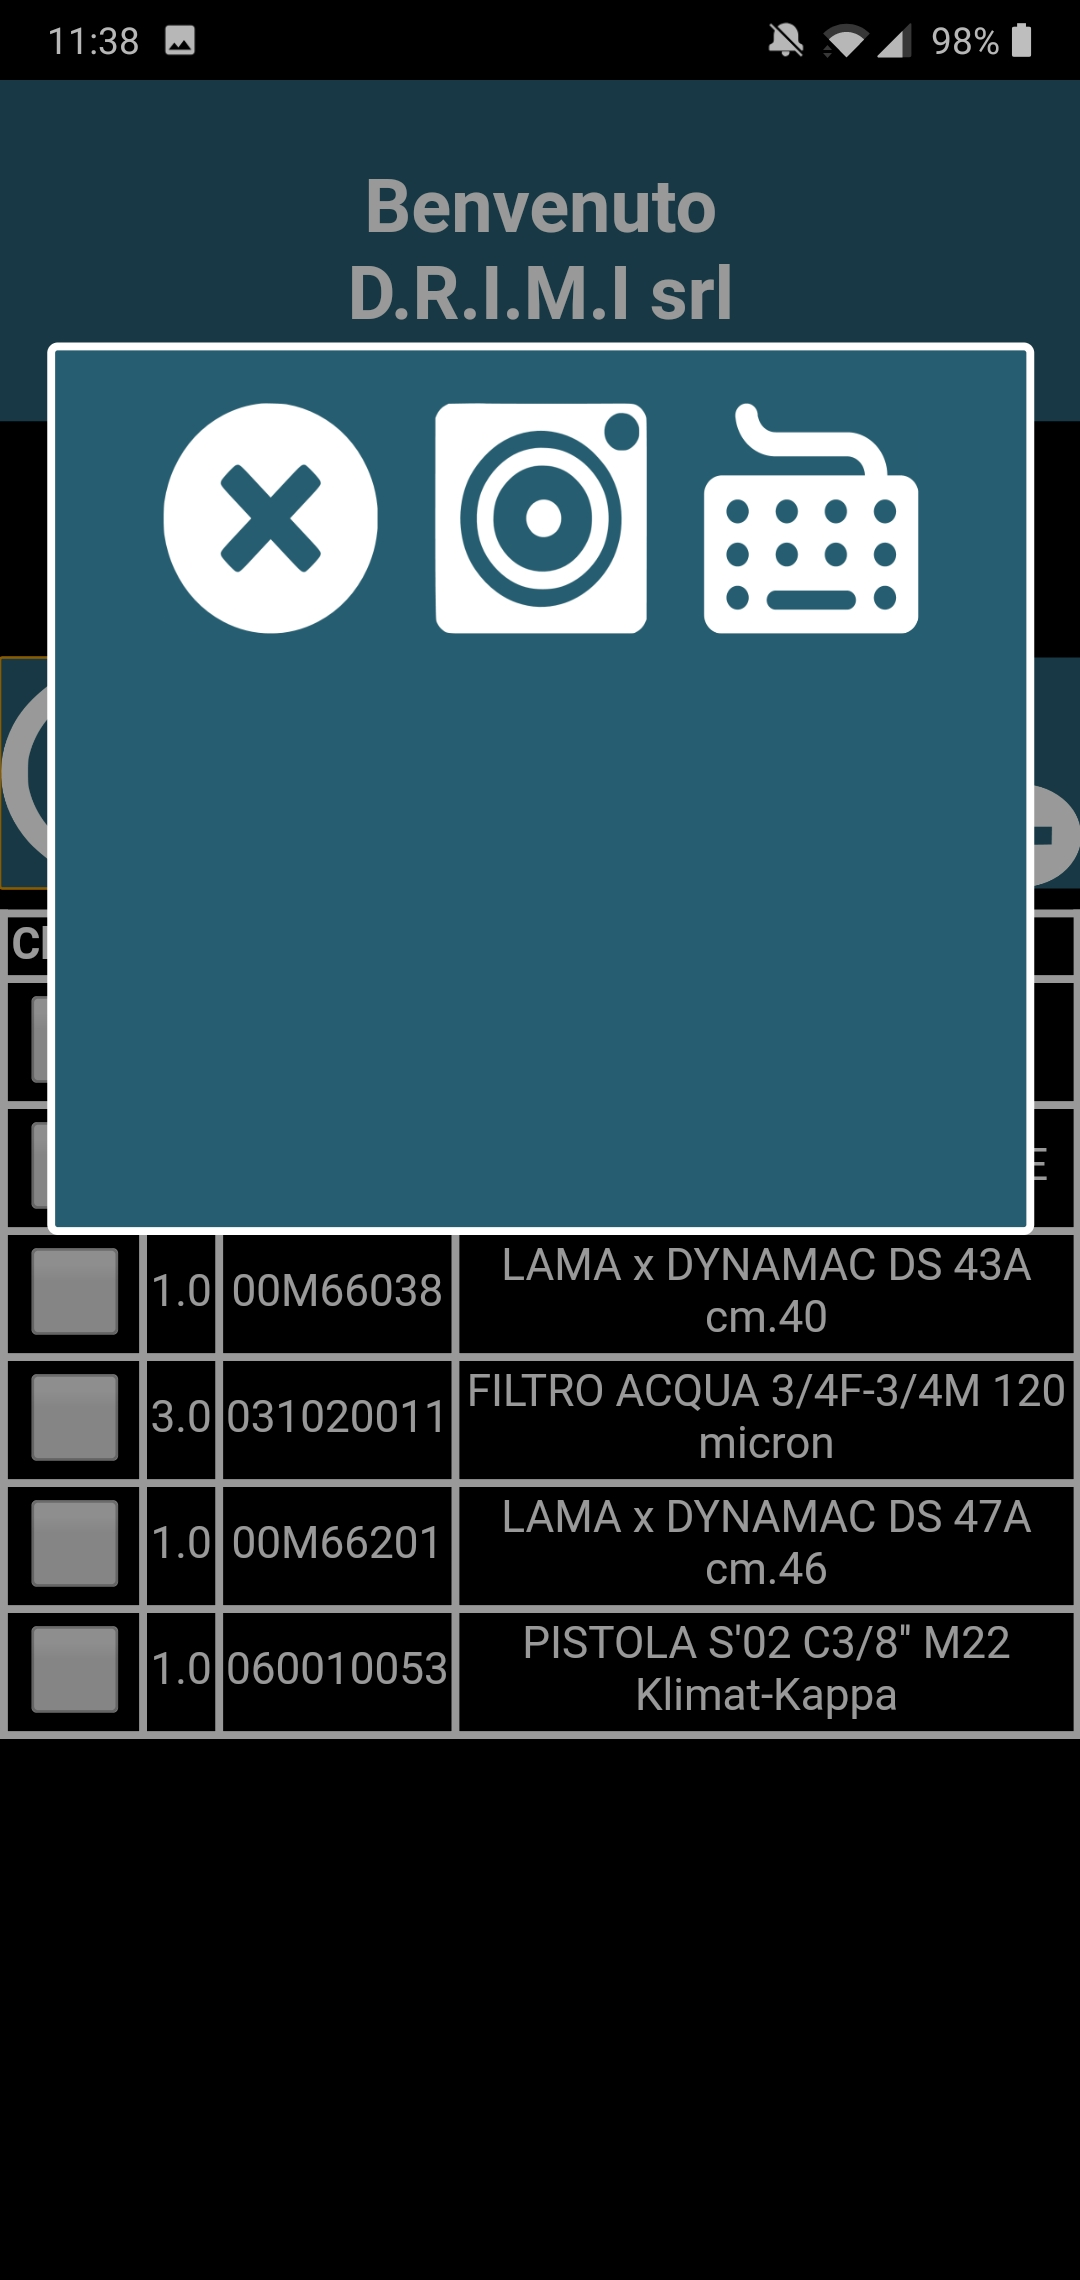
\includegraphics[width=0.33\columnwidth]{interfaccia/modalAggiunta}}
    	\subfloat{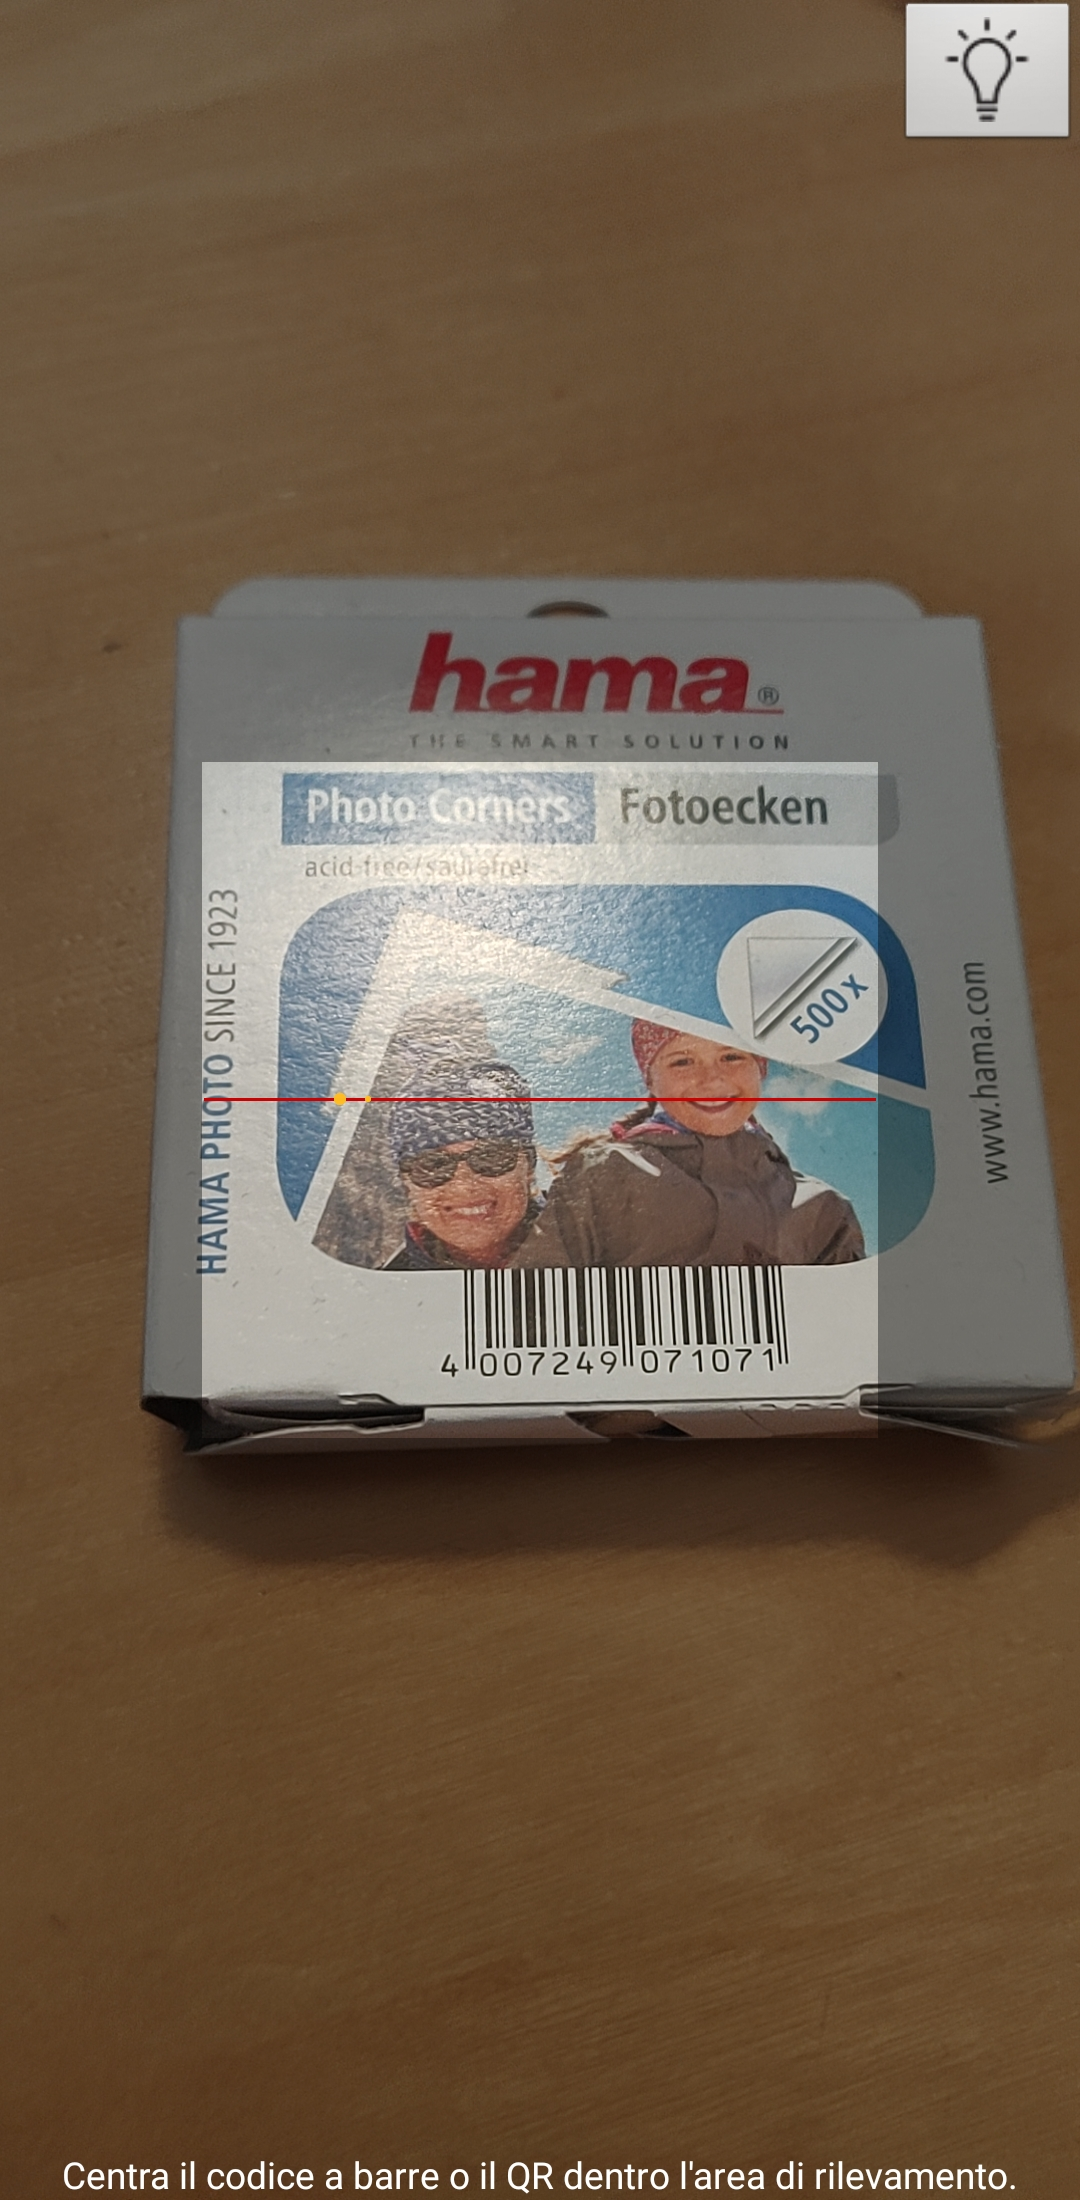
\includegraphics[width=0.33\columnwidth]{interfaccia/scansione}} 
    	\subfloat{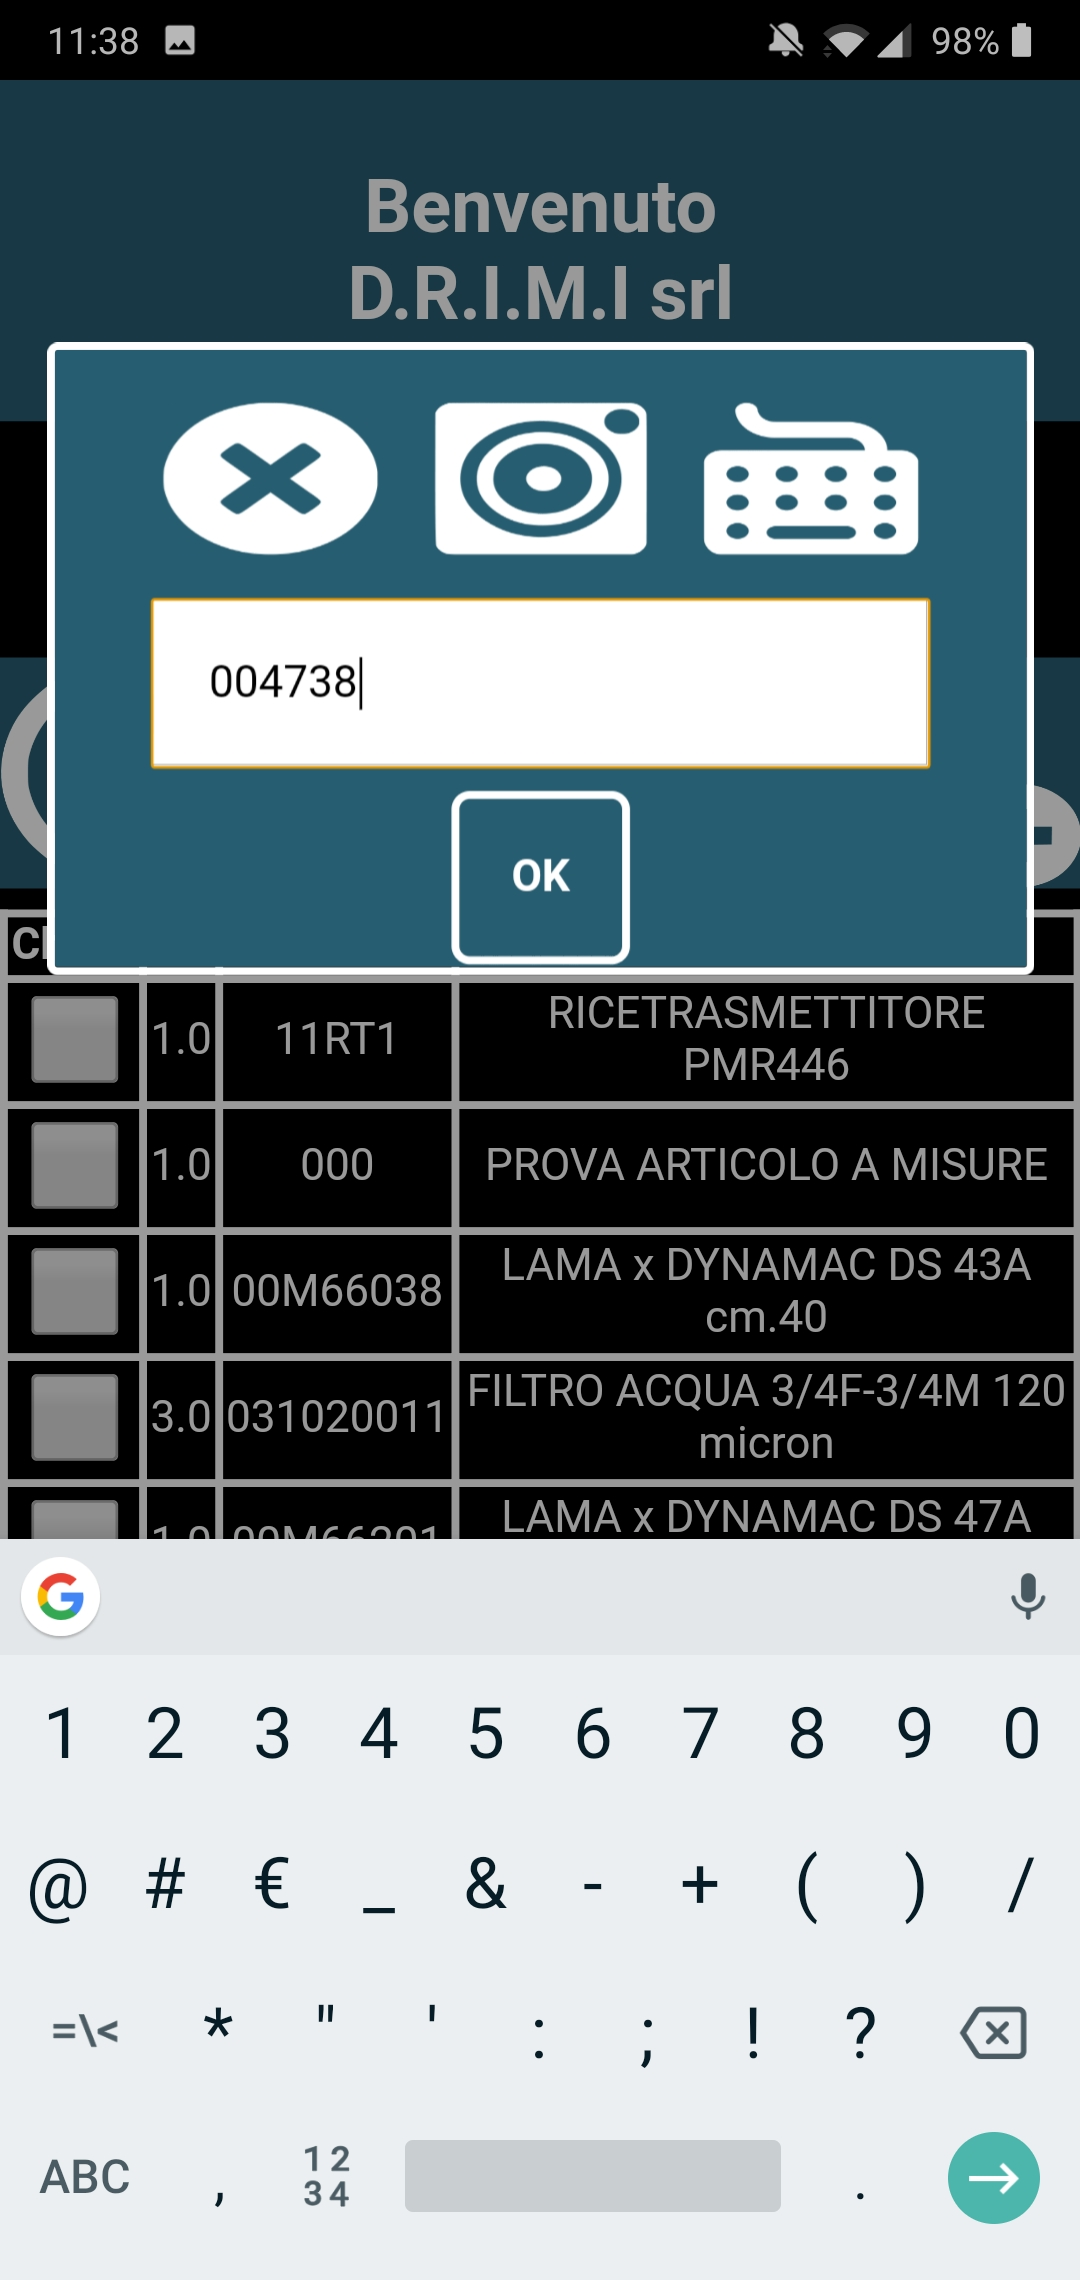
\includegraphics[width=0.33\columnwidth]{interfaccia/manuale}} 
    \caption{\textit{Modal} per l'aggiunta di un articolo e modalità di aggiunta (scansione o inserimento manuale)}
\end{figure}

Il \textit{modal} per l'aggiunta di un articolo permette di decidere la modalità di inserimento dello stesso in carrello. Esso presenta i seguenti pulsanti:
\begin{itemize}
	\item \textbf{annullamento aggiunta}: permette di tornare alla \textit{home page} dell'applicazione;
	\item \textbf{scansione codice a barre}: permette di aggiungere un nuovo articolo scansionando il codice a barre dello stesso. Per effettuare la scansione viene aperta la fotocamera del dispositivo;
	\item \textbf{inserimento manuale}: permette di aggiungere un nuovo articolo inserendo manualmente il codice dello stesso.
\end{itemize}
Se la scansione del \textit{barcode} o l'inserimento del codice vanno a buon fine, viene aperta la pagina per l'aggiunta dell'articolo corrispondente.

\newpage

\subsection{Pagina per l'aggiunta di un articolo}

\begin{figure}[!h] 
    \centering 
    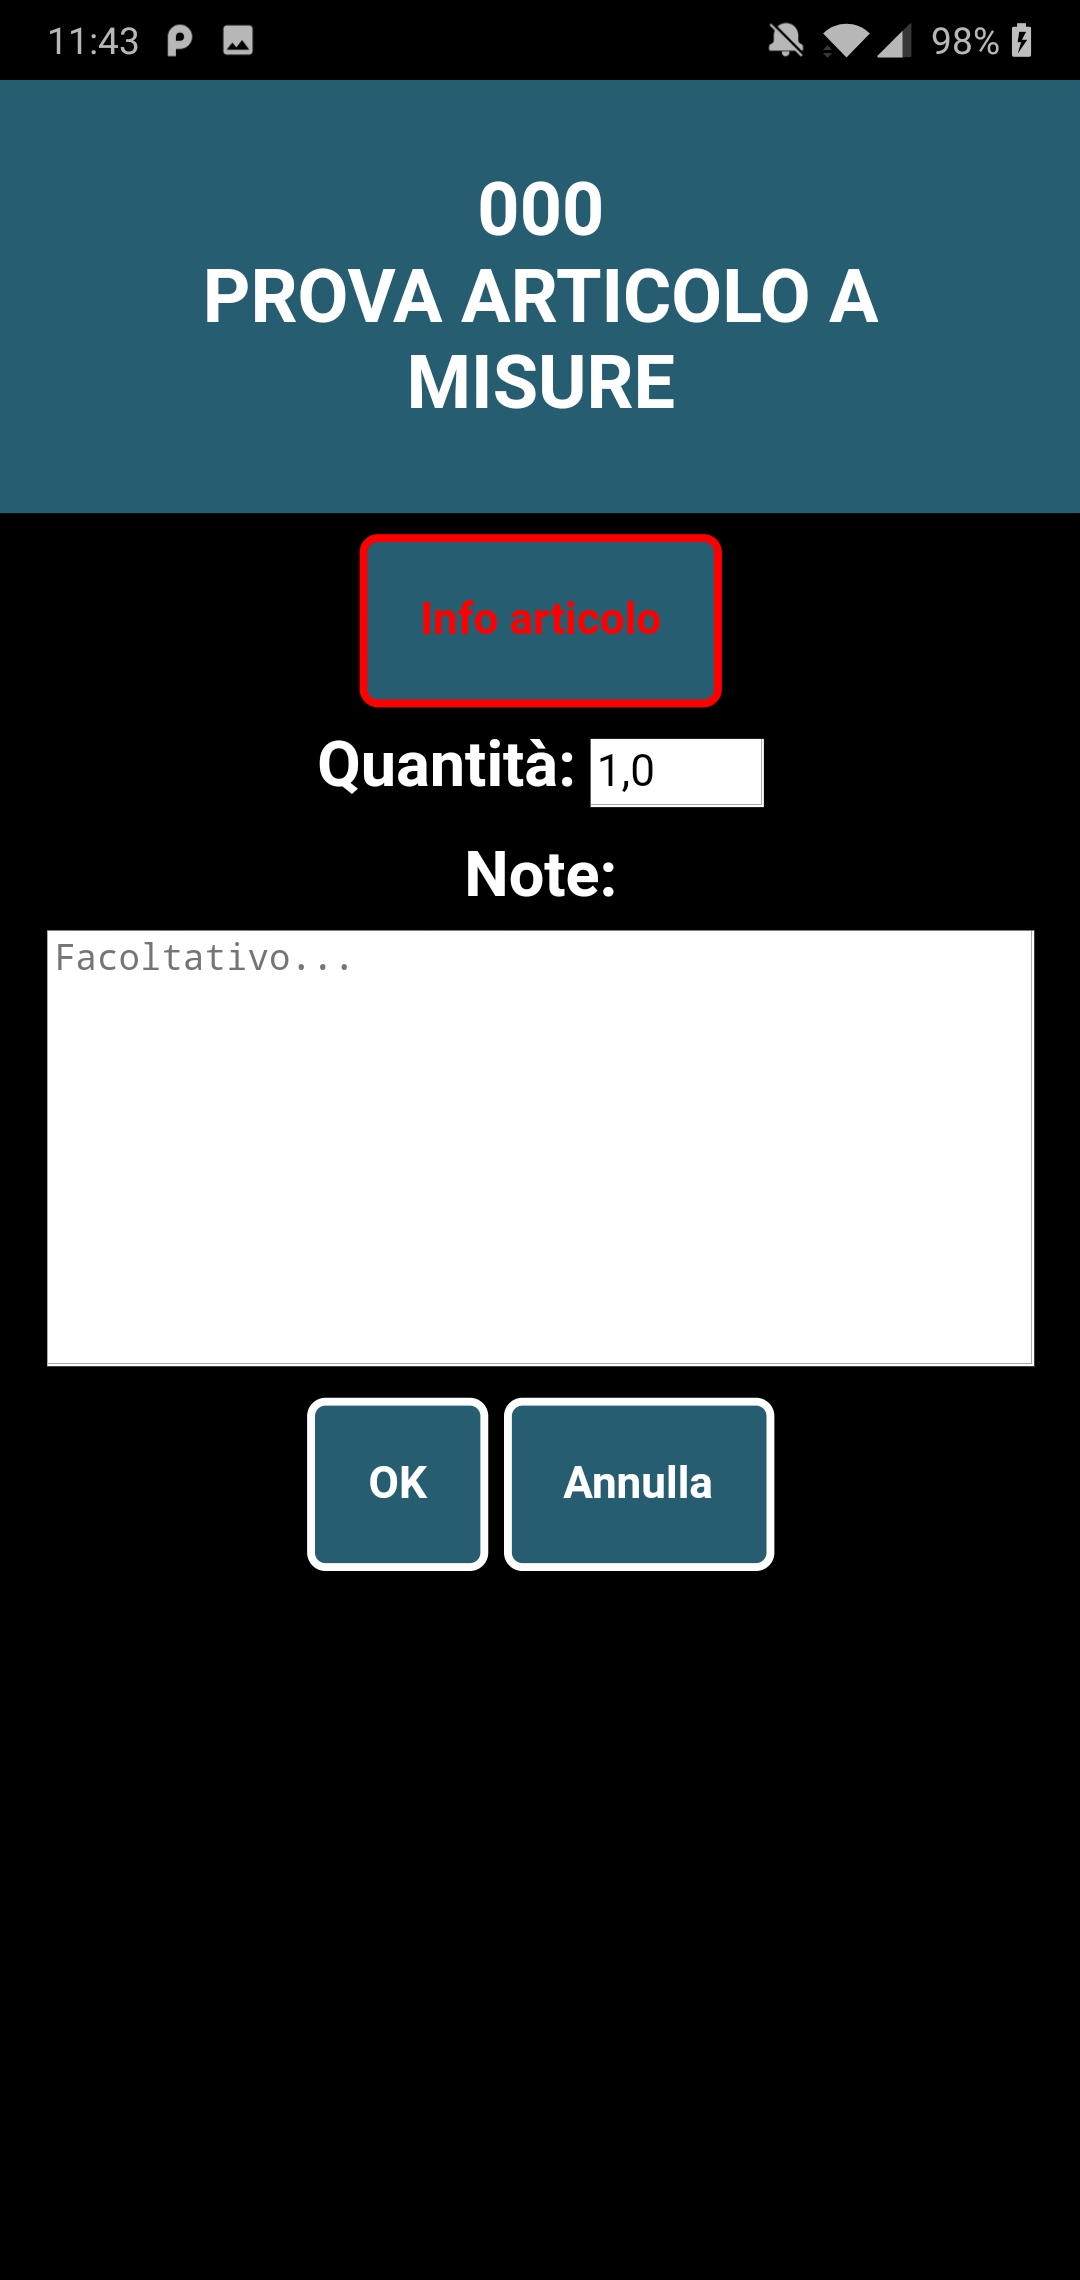
\includegraphics[width=0.4\columnwidth]{interfaccia/aggiunta} 
    \caption{Pagina per l'aggiunta di un articolo}
\end{figure}

La pagina per l'aggiunta di un articolo permette di aggiungere un nuovo articolo al carrello ed è composta dalle seguenti parti:
\begin{itemize}
	\item \textbf{codice e nome dell'articolo}: in base al codice precedentemente scansionato o inserito, vengono visualizzate le informazioni relative al codice e al nome dell'articolo;
	\item \textbf{pulsante di visualizzazione informazioni}: permette di visualizzare le informazioni dell'articolo che si sta aggiungendo al carrello. Per evitare pressioni inutili, il pulsante presenta bordo rosso se per l'articolo non esistono informazioni;
	\item \textbf{\textit{text box} per l'inserimento della quantità}: permette di inserire la quantità dell'articolo che si sta aggiungendo al carrello;
	\item \textbf{\textit{text area} per l'inserimento delle note}: permette di inserire delle note facoltative per l'articolo che si sta aggiungendo al carrello;
	\item \textbf{pulsante di conferma}: permette di confermare l'aggiunta dell'articolo;
	\item \textbf{pulsante di annullamento}: permette di annullare l'aggiunta dell'articolo e di tornare alla \textit{home page} dell'applicazione.
\end{itemize}

\subsection{Pagina per la modifica di un articolo}

Premendo su un qualsiasi articolo in carrello viene aperta una pagina per modificare i dati d'ordine dello stesso. Questa funziona allo stesso modo della pagina per l'aggiunta di un articolo, ma differisce da quest'ultima perché permette invece di modificare l'articolo.

\subsection{\textit{Modal} per l'invio di un ordine}

\begin{figure}[!h] 
    \centering 
    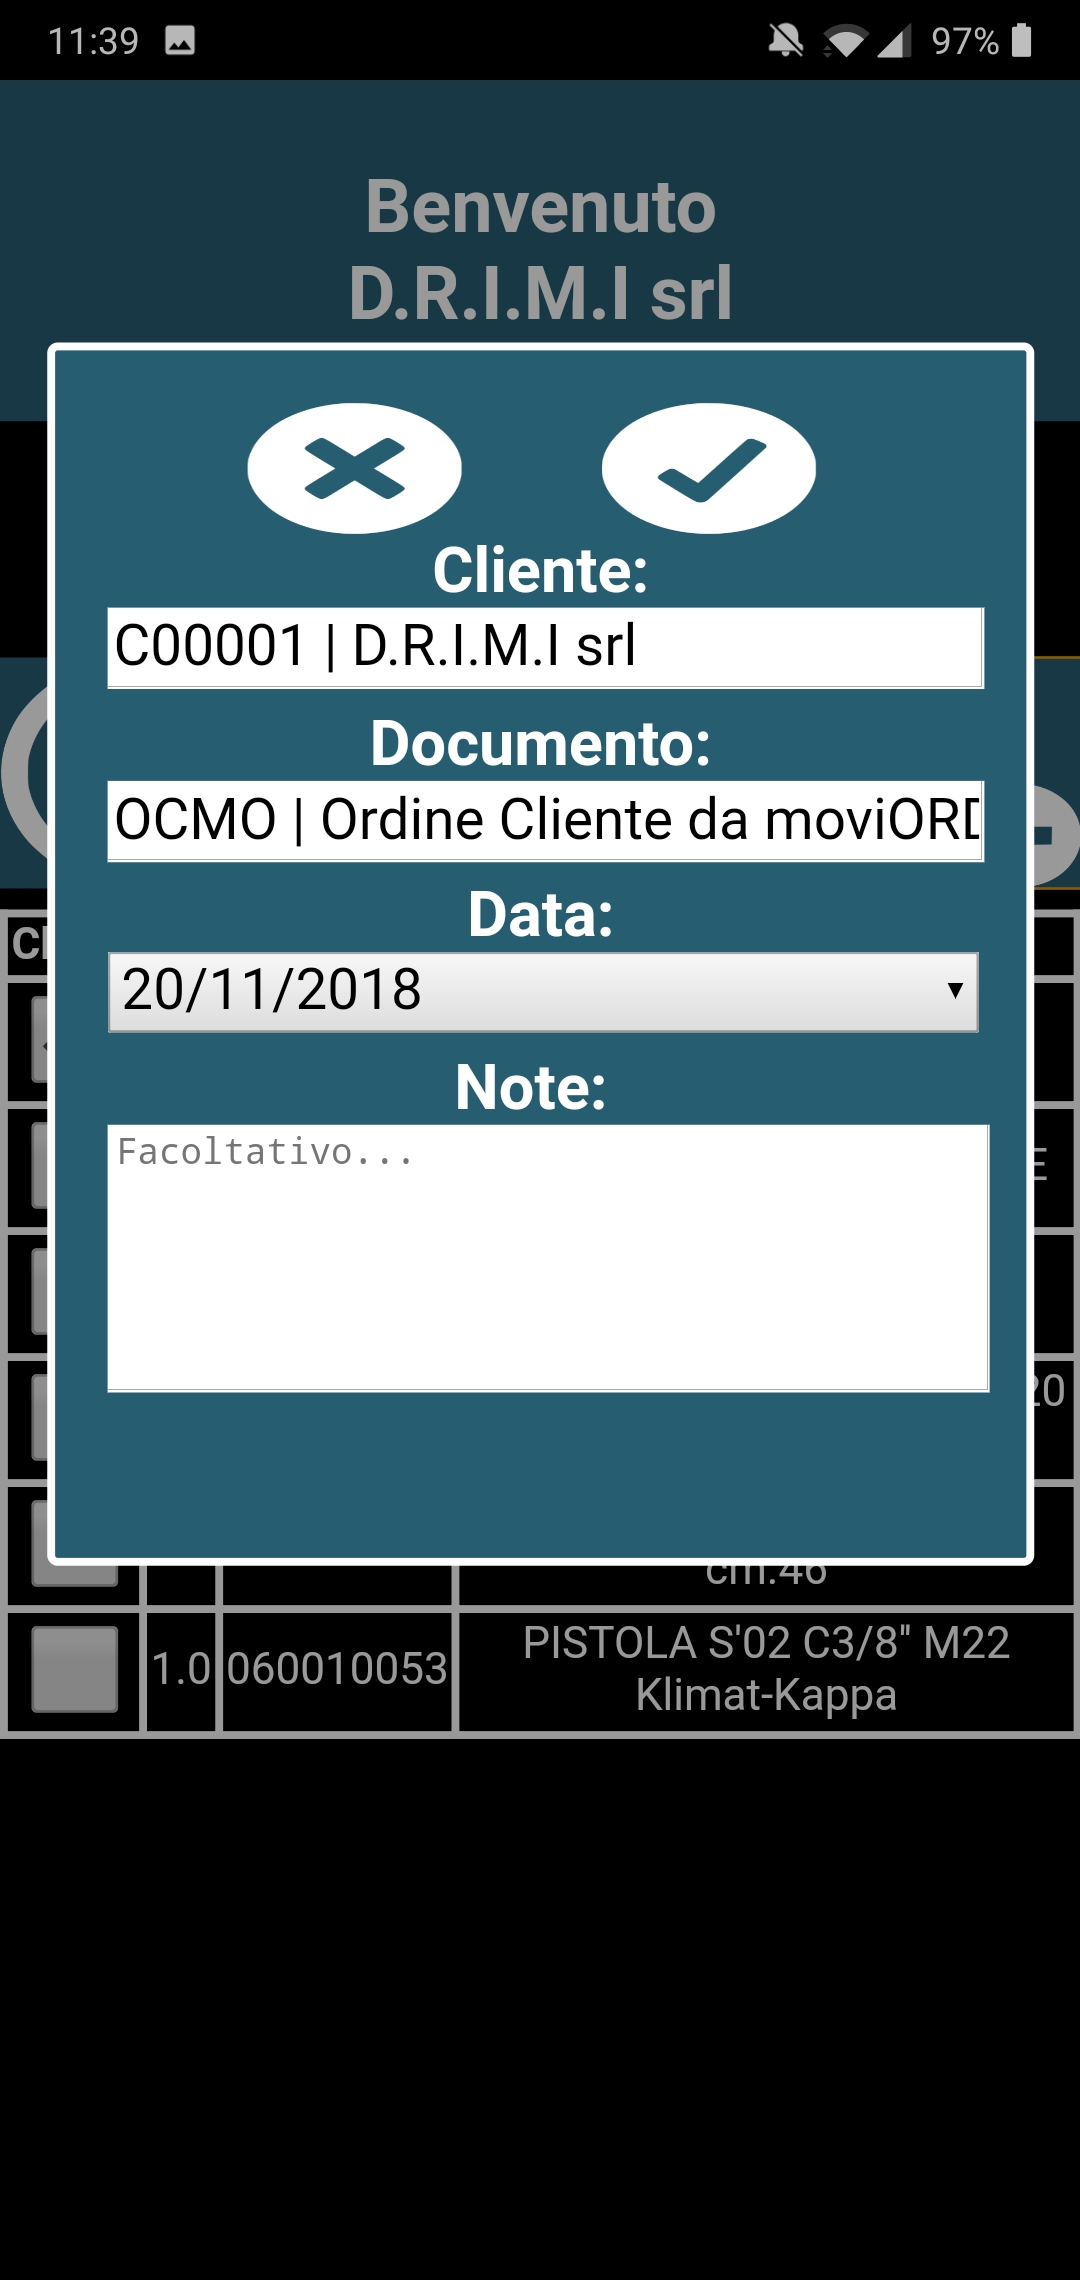
\includegraphics[width=0.4\columnwidth]{interfaccia/modalInvio} 
    \caption{\textit{Modal} per l'invio di un ordine}
\end{figure}

Il \textit{modal} per l'invio di un ordine permette di inviare un ordine all'azienda dell'utente autenticato, contenente tutti gli articoli che lo stesso ha precedentemente selezionato dal carrello. Il \textit{modal} è composto dalle seguenti parti:
\begin{itemize}
	\item \textbf{pulsante di annullamento}: permette di annullare l'invio dell'ordine e di tornare alla \textit{home page} dell'applicazione;
	\item \textbf{pulsante di conferma}: permette di confermare l'invio dell'ordine;
	\item \textbf{informazioni sul cliente}: \textit{text box} contenente il codice e la ragione sociale del cliente che sta effettuando l'ordine;
	\item \textbf{informazioni sul documento}: \textit{text box} contenente il codice e la descrizione del documento che deve essere generato quando viene inviato l'ordine;
	\item \textbf{\textit{select} per l'inserimento della data}: permette di inserire la data dell'ordine. Di \textit{default} viene proposta la data corrente;
	\item \textbf{\textit{text area} per l'inserimento delle note}: permette di inserire delle note facoltative per l'ordine che si sta inviando.
\end{itemize}

\subsection{Considerazioni sullo sviluppo}

L'applicazione è stata realizzata con un \textit{framework cross-platform}, quindi tramite la realizzazione di un'applicazione \textit{web}. Per rendere l'applicazione usabile su tutti gli \textit{smartphone} è stato necessario progettare l'interfaccia con un approccio \glossaryItem{mobile first}, ossia cercando di renderla più \textit{responsive} possibile. Per raggiungere questo obiettivo è stato utilizzato un \glossaryItem{layout elastico}, ossia un \textit{layout} che utilizza unità di misura relative (\textit{em} e \textit{\%}), le quali dipendono dalle preferenze dell'utente. In questo modo le pagine possono adattarsi correttamente ad ogni dimensione di schermo. Viene di seguito fornito, a scopo illustrativo, un esempio di codice \textit{css} che utilizza unità di misura relative.

\begin{figure}[!h] 
    \centering 
    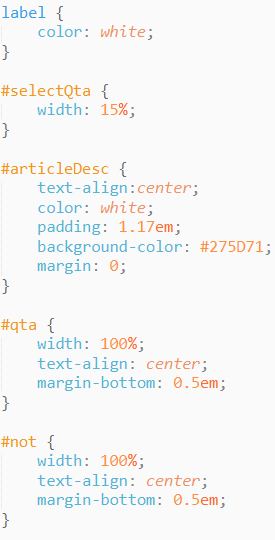
\includegraphics[width=0.5\columnwidth]{codice/css} 
    \caption{Codice \textit{css} che utilizza unità di misura relative}
\end{figure}